% Options for packages loaded elsewhere
\PassOptionsToPackage{unicode}{hyperref}
\PassOptionsToPackage{hyphens}{url}
%
\documentclass[
]{book}
\usepackage{lmodern}
\usepackage{amsmath}
\usepackage{ifxetex,ifluatex}
\ifnum 0\ifxetex 1\fi\ifluatex 1\fi=0 % if pdftex
  \usepackage[T1]{fontenc}
  \usepackage[utf8]{inputenc}
  \usepackage{textcomp} % provide euro and other symbols
  \usepackage{amssymb}
\else % if luatex or xetex
  \usepackage{unicode-math}
  \defaultfontfeatures{Scale=MatchLowercase}
  \defaultfontfeatures[\rmfamily]{Ligatures=TeX,Scale=1}
\fi
% Use upquote if available, for straight quotes in verbatim environments
\IfFileExists{upquote.sty}{\usepackage{upquote}}{}
\IfFileExists{microtype.sty}{% use microtype if available
  \usepackage[]{microtype}
  \UseMicrotypeSet[protrusion]{basicmath} % disable protrusion for tt fonts
}{}
\makeatletter
\@ifundefined{KOMAClassName}{% if non-KOMA class
  \IfFileExists{parskip.sty}{%
    \usepackage{parskip}
  }{% else
    \setlength{\parindent}{0pt}
    \setlength{\parskip}{6pt plus 2pt minus 1pt}}
}{% if KOMA class
  \KOMAoptions{parskip=half}}
\makeatother
\usepackage{xcolor}
\IfFileExists{xurl.sty}{\usepackage{xurl}}{} % add URL line breaks if available
\IfFileExists{bookmark.sty}{\usepackage{bookmark}}{\usepackage{hyperref}}
\hypersetup{
  pdftitle={Introducción a la Programación},
  pdfauthor={Mgs. Lic. Marcos Prunello (Prof.~Tit. Ord.)},
  hidelinks,
  pdfcreator={LaTeX via pandoc}}
\urlstyle{same} % disable monospaced font for URLs
\usepackage{color}
\usepackage{fancyvrb}
\newcommand{\VerbBar}{|}
\newcommand{\VERB}{\Verb[commandchars=\\\{\}]}
\DefineVerbatimEnvironment{Highlighting}{Verbatim}{commandchars=\\\{\}}
% Add ',fontsize=\small' for more characters per line
\usepackage{framed}
\definecolor{shadecolor}{RGB}{248,248,248}
\newenvironment{Shaded}{\begin{snugshade}}{\end{snugshade}}
\newcommand{\AlertTok}[1]{\textcolor[rgb]{0.94,0.16,0.16}{#1}}
\newcommand{\AnnotationTok}[1]{\textcolor[rgb]{0.56,0.35,0.01}{\textbf{\textit{#1}}}}
\newcommand{\AttributeTok}[1]{\textcolor[rgb]{0.77,0.63,0.00}{#1}}
\newcommand{\BaseNTok}[1]{\textcolor[rgb]{0.00,0.00,0.81}{#1}}
\newcommand{\BuiltInTok}[1]{#1}
\newcommand{\CharTok}[1]{\textcolor[rgb]{0.31,0.60,0.02}{#1}}
\newcommand{\CommentTok}[1]{\textcolor[rgb]{0.56,0.35,0.01}{\textit{#1}}}
\newcommand{\CommentVarTok}[1]{\textcolor[rgb]{0.56,0.35,0.01}{\textbf{\textit{#1}}}}
\newcommand{\ConstantTok}[1]{\textcolor[rgb]{0.00,0.00,0.00}{#1}}
\newcommand{\ControlFlowTok}[1]{\textcolor[rgb]{0.13,0.29,0.53}{\textbf{#1}}}
\newcommand{\DataTypeTok}[1]{\textcolor[rgb]{0.13,0.29,0.53}{#1}}
\newcommand{\DecValTok}[1]{\textcolor[rgb]{0.00,0.00,0.81}{#1}}
\newcommand{\DocumentationTok}[1]{\textcolor[rgb]{0.56,0.35,0.01}{\textbf{\textit{#1}}}}
\newcommand{\ErrorTok}[1]{\textcolor[rgb]{0.64,0.00,0.00}{\textbf{#1}}}
\newcommand{\ExtensionTok}[1]{#1}
\newcommand{\FloatTok}[1]{\textcolor[rgb]{0.00,0.00,0.81}{#1}}
\newcommand{\FunctionTok}[1]{\textcolor[rgb]{0.00,0.00,0.00}{#1}}
\newcommand{\ImportTok}[1]{#1}
\newcommand{\InformationTok}[1]{\textcolor[rgb]{0.56,0.35,0.01}{\textbf{\textit{#1}}}}
\newcommand{\KeywordTok}[1]{\textcolor[rgb]{0.13,0.29,0.53}{\textbf{#1}}}
\newcommand{\NormalTok}[1]{#1}
\newcommand{\OperatorTok}[1]{\textcolor[rgb]{0.81,0.36,0.00}{\textbf{#1}}}
\newcommand{\OtherTok}[1]{\textcolor[rgb]{0.56,0.35,0.01}{#1}}
\newcommand{\PreprocessorTok}[1]{\textcolor[rgb]{0.56,0.35,0.01}{\textit{#1}}}
\newcommand{\RegionMarkerTok}[1]{#1}
\newcommand{\SpecialCharTok}[1]{\textcolor[rgb]{0.00,0.00,0.00}{#1}}
\newcommand{\SpecialStringTok}[1]{\textcolor[rgb]{0.31,0.60,0.02}{#1}}
\newcommand{\StringTok}[1]{\textcolor[rgb]{0.31,0.60,0.02}{#1}}
\newcommand{\VariableTok}[1]{\textcolor[rgb]{0.00,0.00,0.00}{#1}}
\newcommand{\VerbatimStringTok}[1]{\textcolor[rgb]{0.31,0.60,0.02}{#1}}
\newcommand{\WarningTok}[1]{\textcolor[rgb]{0.56,0.35,0.01}{\textbf{\textit{#1}}}}
\usepackage{longtable,booktabs}
\usepackage{calc} % for calculating minipage widths
% Correct order of tables after \paragraph or \subparagraph
\usepackage{etoolbox}
\makeatletter
\patchcmd\longtable{\par}{\if@noskipsec\mbox{}\fi\par}{}{}
\makeatother
% Allow footnotes in longtable head/foot
\IfFileExists{footnotehyper.sty}{\usepackage{footnotehyper}}{\usepackage{footnote}}
\makesavenoteenv{longtable}
\usepackage{graphicx}
\makeatletter
\def\maxwidth{\ifdim\Gin@nat@width>\linewidth\linewidth\else\Gin@nat@width\fi}
\def\maxheight{\ifdim\Gin@nat@height>\textheight\textheight\else\Gin@nat@height\fi}
\makeatother
% Scale images if necessary, so that they will not overflow the page
% margins by default, and it is still possible to overwrite the defaults
% using explicit options in \includegraphics[width, height, ...]{}
\setkeys{Gin}{width=\maxwidth,height=\maxheight,keepaspectratio}
% Set default figure placement to htbp
\makeatletter
\def\fps@figure{htbp}
\makeatother
\setlength{\emergencystretch}{3em} % prevent overfull lines
\providecommand{\tightlist}{%
  \setlength{\itemsep}{0pt}\setlength{\parskip}{0pt}}
\setcounter{secnumdepth}{5}
% \usepackage{booktabs}
% \usepackage{amsthm}
% \usepackage{amssymb}
\usepackage{booktabs}
\usepackage{multirow}

\usepackage[spanish]{babel}
\usepackage[utf8]{inputenc}
\spanishdecimal{.}
%\renewcommand{\contentsname}{Contenido}


% Encabezado
\usepackage[margin=2cm]{geometry}
\usepackage{fancyhdr}
\pagestyle{fancy}
\renewcommand{\footrulewidth}{0.4pt}
\renewcommand{\sectionmark}[1]{\markright{#1}}
\fancyhead[L]{IALP - Guía de Estudio}
\fancyhead[R] {\leftmark}

% Formato para el capítulo
% Para que diga Unidad en lugar de Capítulo
\makeatletter
\renewcommand{\@chapapp}{Unidad}
\makeatother
% Para que diga "Unidad" antes del nro y nombre de la unidad
%\usepackage{titlesec}
%\titleformat{\chapter}{
%	\normalfont\LARGE\bfseries
%}{Unidad \thechapter.  }{0em}{}

% Para que haya encabezado en la primera hoja de cada cap tmb
\usepackage{etoolbox}
\patchcmd{\chapter}{\thispagestyle{plain}}{\thispagestyle{fancy}}{}{}

% Pero lo anterior agrega encabezad en la tabla de contenidos, esto lo evita
\AtBeginDocument{%
	\addtocontents{toc}{\protect\thispagestyle{empty}}
}

% Agregar puntos en el TOC en el nivel de capitulo
\usepackage{tocloft}
\renewcommand{\cftchapleader}{\cftdotfill{\cftdotsep}} % for chapters

% Info para la portada
\newcommand{\horrule}[1]{\rule{\linewidth}{#1}}
\title{
	%\vspace{-1in} 	
	\usefont{OT1}{bch}{b}{n}
	\normalfont \normalsize
	\textsc{
		Universidad Nacional de Rosario \\
		Facultad de Ciencias Económicas y Estadística \\
		Licenciatura en Estadística
	} \\ [25pt]
	\horrule{2pt} \\[0.4cm]
	\huge \textbf{Introducción a la Programación} \\
	\bigbreak
	Guía de Estudio - Año 2021\\
	\horrule{2pt} \\[0.5cm]}

\author{
	\normalfont Mgs. Lic. Marcos Prunello (Prof. Tit. Ordenado)
}

% Esto es para que el cuadro sombreado donde sale el codigo sea mas chico y para que el espacio entre el codigo y el output sea menor
\usepackage{etoolbox,framed} 
\setlength{\parskip}{2pt}
\setlength{\OuterFrameSep}{2pt}
\makeatletter
\preto{\@verbatim}{\topsep=2pt \partopsep=2pt }
\makeatother

% Otros paquetes
\usepackage{xcolor}

% cosas para modificar espacios entre ecuaciones y otros
% Que haya menos espacio antes y dps de ecuaciones
% \usepackage{setspace}\onehalfspacing
% \AtBeginDocument{%
%   % estas dos 
%   %\addtolength\abovedisplayskip{-0.5\baselineskip}%
%   %\addtolength\belowdisplayskip{-0.5\baselineskip}
%   % o estas dos, probar cual me gusta mas
%   \setlength{\belowdisplayskip}{0pt} \setlength{\belowdisplayshortskip}{0pt}
%   \setlength{\abovedisplayskip}{0pt} \setlength{\abovedisplayshortskip}{0pt}
% }
% 
% \setlength{\intextsep}{0pt}
% 
% \makeatletter
% \def\thm@space@setup{%
%   \thm@preskip=8pt plus 2pt minus 4pt
%   \thm@postskip=\thm@preskip
% }
% \makeatother

% Columnas
\newenvironment{columns}[1][]{}{}

\newenvironment{column}[1]{\begin{minipage}{#1}\ignorespaces}{%
\end{minipage}
\ifhmode\unskip\fi
\aftergroup\useignorespacesandallpars}

\def\useignorespacesandallpars#1\ignorespaces\fi{%
#1\fi\ignorespacesandallpars}

\makeatletter
\def\ignorespacesandallpars{%
  \@ifnextchar\par
    {\expandafter\ignorespacesandallpars\@gobble}%
    {}%
}
\makeatother

% Para que en Latex las tables queden donde quiero
\usepackage{float}
% \floatplacement{table}{H}
\ifluatex
  \usepackage{selnolig}  % disable illegal ligatures
\fi
\usepackage[]{natbib}
\bibliographystyle{plainnat}

\title{Introducción a la Programación}
\usepackage{etoolbox}
\makeatletter
\providecommand{\subtitle}[1]{% add subtitle to \maketitle
  \apptocmd{\@title}{\par {\large #1 \par}}{}{}
}
\makeatother
\subtitle{Guía de estudio - Lic. en Estadística - FCEyE - UNR}
\author{Mgs. Lic. Marcos Prunello (Prof.~Tit. Ord.)}
\date{2021-05-13}

\begin{document}
\maketitle

{
\setcounter{tocdepth}{1}
\tableofcontents
}
\newpage

\textbf{BIENVENIDA}

\vspace{\baselineskip}

¡Les damos la bienvenida a la asignatura Introducción a la Programación en la Facultad de Ciencias Económicas y Estadística, Universidad Nacional de Rosario! La presente guía resume los conceptos más importantes que vamos a desarrollar. La misma irá siendo revisada, completada y actualizada a lo largo del cuatrimestre y no está exenta de presentar errores o expresar ideas que puedan ser mejoradas. Avisanos si encontrás algo que deba ser cambiado. ¡Esperamos que juntos podamos pasarla bien al dar nuestros primeros pasos en la programación!

\vspace{\baselineskip}

Este material fue escrito por el Mgs. Lic. Marcos Prunello (profesor titular) y revisado por los integrantes de la cátedra, Tec. César Mignoni y Lic. Maite San Martín.

\vspace{\baselineskip}

\textbf{NOTA: La versión en PDF no es revisada en cuanto a su configuración, por lo tanto es probable que se encuentren páginas con espacios en blanco, tablas con filas cortadas, figuras muy grandes, etc. El archivo PDF es generado sin revisar su estado final, pero el texto es el mismo que la versión online (\url{https://mpru.github.io/introprog})}

\hypertarget{introducciuxf3n-a-la-programaciuxf3n}{%
\chapter{Introducción a la Programación}\label{introducciuxf3n-a-la-programaciuxf3n}}

\hypertarget{quuxe9-es-la-programaciuxf3n}{%
\section{Qué es la programación}\label{quuxe9-es-la-programaciuxf3n}}

Las computadoras son una parte esencial de nuestra vida cotidiana. Casi todos los aparatos que usamos tienen algún tipo de computadora capaz de ejecutar ciertas tareas: lavarropas con distintos modos de lavado, consolas de juegos para momentos de entretenimiento, calculadoras súper potentes, computadoras personales que se usan para un montón de propósitos, teléfonos celulares con un sinfín de aplicaciones y miles de cosas más.

Todos estos dispositivos con computadoras de distinto tipo tienen algo en común: alguien ``les dice'' cómo funcionar, es decir, les indica cuáles son los pasos que deben seguir para cumplir una tarea. De eso se trata la \emph{programación}: es la actividad mediante la cual las \emph{personas} le entregan a una \emph{computadora} un conjunto de instrucciones para que, al ejecutarlas, ésta pueda \emph{resolver un problema}. Quienes realizan esta actividad reciben el nombre de \emph{programadores}. Sin las personas que las programen, las computadoras dejan de ser útiles, por más complejos que sean estos aparatos. Los conjuntos de instrucciones que reciben las computadoras reciben el nombre de \emph{programas}.

La programación es un proceso creativo: en muchas ocasiones la tarea en cuestión puede cumplirse siguiendo distintos caminos y el programador es el que debe imaginar cuáles son y elegir uno. Algunos de estos caminos pueden ser mejores que otros, pero en cualquier caso la computadora se limitará a seguir las instrucciones ideadas por el programador.

Desafortunadamente, las computadoras no entienden español ni otro idioma humano. Hay que pasarles las instrucciones en un lenguaje que sean capaces de entender. Para eso debemos aprender algún \emph{lenguaje de programación}, que no es más que un lenguaje artificial compuesto por una serie de expresiones que la computadora puede interpretar. Las computadoras interpretan nuestras instrucciones de forma muy literal, por lo tanto a la hora de programar hay que ser muy específicos. Es necesario respetar las reglas del lenguaje de programación y ser claros en las indicaciones provistas.

Ahora bien, ¿por qué debemos estudiar programación en la Licenciatura en Estadística? La actividad de los profesionales estadísticos está atravesada en su totalidad por la necesidad de manejar con soltura herramientas informáticas que nos asisten en las distintas etapas de nuestra labor, desde la recolección y depuración de conjuntos de datos, pasando por la aplicación de distintas metodologías de análisis, hasta la comunicación efectiva de los resultados. Por eso, en la asignatura \emph{Introducción a la Programación} estudiaremos los conceptos básicos de esta disciplina, fomentando la ejercitación del pensamiento abstracto y lógico necesario para poder entendernos hábilmente con la computadora y lograr que la misma realice las tareas que necesitamos.

Para poner en práctica los conceptos sobre Programación que aprenderemos, vamos a emplear un lenguaje que ha sido desarrollado específicamente para realizar tareas estadísticas, llamado \emph{R}. Sin embargo, debemos resaltar que éste no es un curso sobre R, es decir, no nos dedicaremos a aprender las herramientas que este lenguaje brinda para el análisis de datos. De hecho, frente a variados problemas vamos a dedicarnos a crear soluciones que ya existen y están disponibles en R, pero lo haremos con el fin de utilizar dicho lenguaje para aprender y ejercitar nociones básicas de programación.

\hypertarget{una-breve-reseuxf1a-histuxf3rica-sobre-la-programaciuxf3n}{%
\section{Una breve reseña histórica sobre la programación}\label{una-breve-reseuxf1a-histuxf3rica-sobre-la-programaciuxf3n}}

La historia de la programación está vinculada directamente con la de la computación. Esta palabra proviene del latín \emph{computatio}, que deriva del verbo \emph{computare}, cuyo significado es ``enumerar cantidades''. Computación, en este sentido, designa la acción y efecto de computar, realizar una cuenta, un cálculo matemático. De allí que antiguamente computación fuese un término usado para referirse a los cálculos realizados por una persona con un instrumento expresamente utilizado para tal fin (como el ábaco, por ejemplo) o sin él. En este sentido, la computación ha estado presente desde tiempos ancestrales, sin embargo debemos remontarnos al siglo XVII para encontrar los primeros dispositivos diseñados para automatizar cómputos matemáticos.

En 1617 el matemático escocés John Napier (el mismo que definió los logaritmos) inventó un sistema conocido como \emph{los huesos de Napier} o \emph{huesos neperianos} que facilitaba la tarea de multiplicar, dividir y tomar raíces cuadradas, usando unas barras de hueso o marfil que tenían dígitos grabados. Esta fue la base para otras ideas más avanzadas, entre ellas la que dio origen a la primera calculadora mecánica, inventada por el alemán Wilhelm Schickard en 1623, capaz de realizar cómputos aritméticos sencillos funcionando a base de ruedas y engranajes. Se componía de dos mecanismos diferenciados, un ábaco de Napier de forma cilíndrica en la parte superior y un mecanismo en la inferior para realizar sumas parciales de los resultados obtenidos con el aparato de la parte superior. Fue llamado \emph{reloj calculador}. A partir de aquí se fueron desarrollando otros modelos, todos ellos teniendo en común el hecho de ser puramente mecánicos, sin motores ni otras fuentes de energía. El operador ingresaba números ubicando ruedas de metal en posiciones particulares y al girarlas otras partes de la máquina se movían y mostraban el resultado. Algunos ejemplos son las calculadoras del inglés William Oughtred en 1624, de Blaise Pascal en 1645 (llamada \emph{pascalina}), la de Samuel Morland en 1666 y las de Leibniz, en 1673 y 1694.

\begin{figure}

{\centering 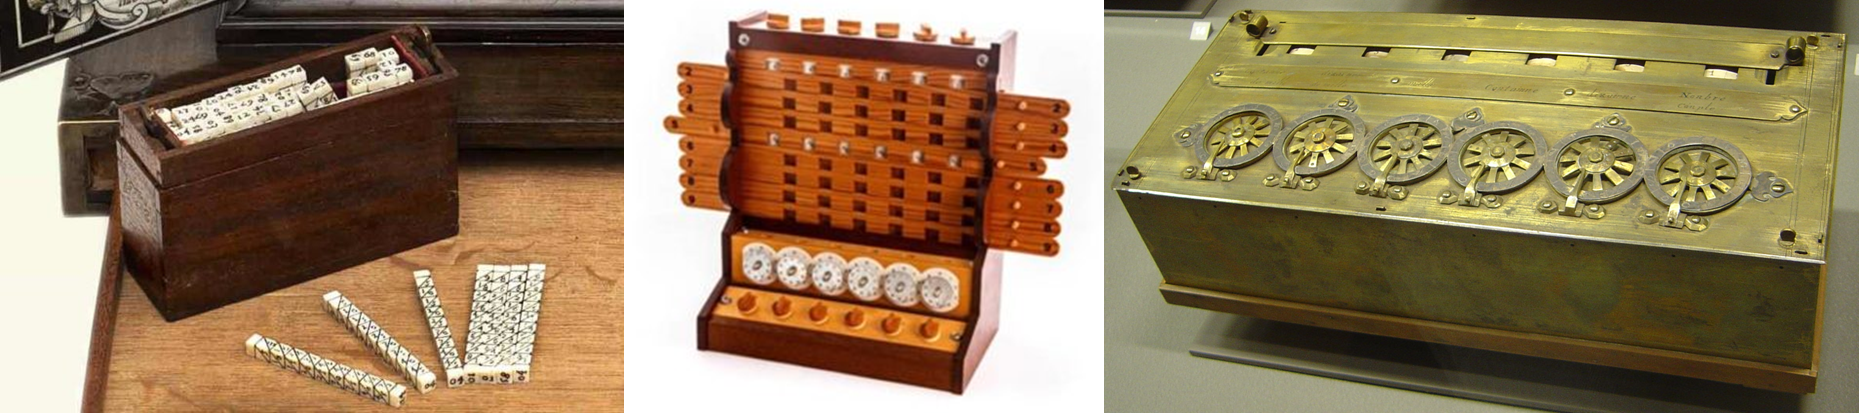
\includegraphics[width=1\linewidth]{images/historia/calculadoras} 

}

\caption{De izquierda a derecha: los huesos de Napier (Museo Arqueológico Nacional de España), el reloj calculador de Schickard (Museo de la Ciencia de la Universidad Pública de Navarra) y una pascalina del año 1952}\label{fig:calculadora}
\end{figure}

El siglo XVIII trajo consigo algunos otros diseños, pero un gran salto se dio a comienzos del siglo XIX de mano de un tejedor y comerciante francés, Joseph Jacquard. En 1801 creó un telar que tenía un sistema de tarjetas perforadas para controlar las puntadas del tejido, de forma que fuera posible \emph{programar} una gran diversidad de tramas y figuras. Sin saberlo, Jacquard sentó una idea fundamental para la creación de las computadoras.

\begin{figure}

{\centering 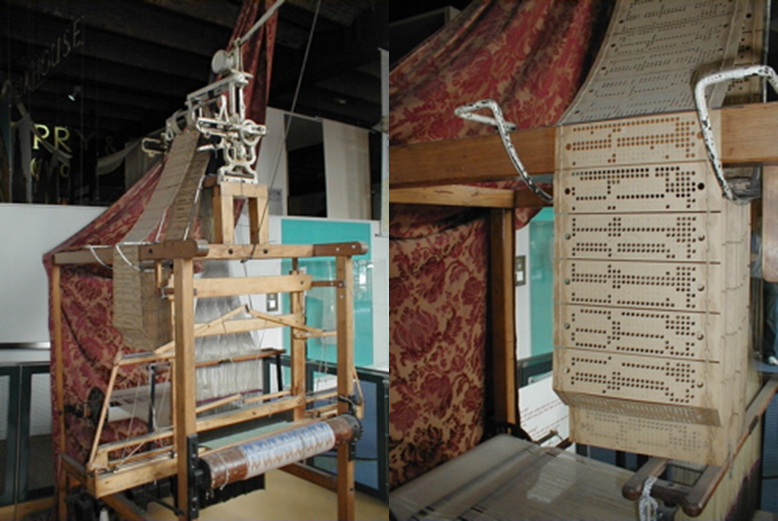
\includegraphics[width=0.5\linewidth]{images/historia/telar} 

}

\caption{Un telar de Jacquard y sus tarjetas perforadas en el Museo de la ciencia y la industria en Mánchester.}\label{fig:unnamed-chunk-1}
\end{figure}

En 1822 el matemático británico Charles Babbage publicó un diseño para la construcción de una \emph{máquina diferencial}, que podía calcular valores de funciones polinómicas mediante el método de las diferencias. Este complejo sistema de ruedas y engranajes era el primero que podía trabajar automáticamente utilizando resultados de operaciones previas. Si bien el diseño era viable, por motivos técnicos y económicos no lo pudo concretar (sólo construyó un modelo de menor escala). Sin embargo, Babbage no se dio por vencido y en 1837 presentó el diseño de una \emph{máquina analítica}, un aparato capaz de ejecutar cualquier tipo de cálculo matemático y que, por lo tanto, se podría utilizar con cualquier propósito. Tal como el telar de Jacquard, la operación de esta máquina sería controlada por un patrón de perforaciones hechas sobre una tarjetas que la misma podría leer. Al cambiar el patrón de las perforaciones, se podría cambiar el comportamiento de la máquina para que resuelva diferentes tipos de cálculos. Para la salida de resultados, la máquina sería capaz de perforar tarjetas. Además, funcionaría con un motor a vapor y su tamaño hubiese sido de 30 metros de largo por 10 de ancho. Si bien Babbage tampoco llegó a concretar en vida este diseño que dejó plasmado en más de 300 dibujos y 2200 páginas por motivos políticos, se lo considera como la primera conceptualización de lo que hoy conocemos como computadora, por lo cual Babbage es conocido como \emph{el padre de la computación}.

En 1843 Lady Ada Lovelace, una matemática y escritora británica, publicó una serie de notas sobre la máquina analítica de Babbage, en las que resaltaba sus potenciales aplicaciones prácticas, incluyendo la descripción detallada de tarjetas perforadas para que sea capaz de calcular los números de Bernoulli. Al haber señalado los pasos para que la máquina pueda cumplir con estas y otras tareas, Ada es considerada actualmente como la primera programadora del mundo, a pesar de que en la época no fue tomada en serio por la comunidad científica, principalmente por su condición de mujer.

\begin{figure}

{\centering 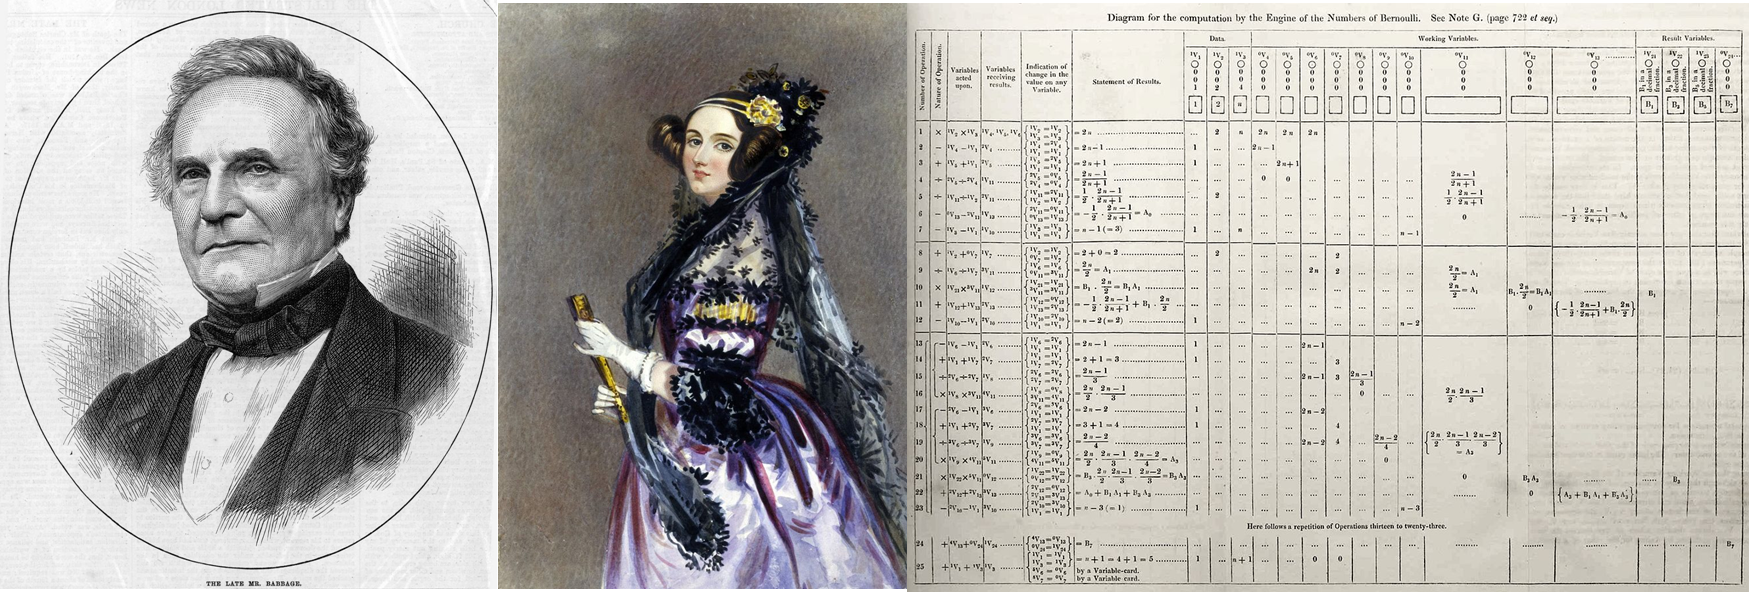
\includegraphics[width=1\linewidth]{images/historia/babbage_ada} 

}

\caption{Charles Babbage, Ada Lovelace y el algoritmo que publicó Ada para calcular los números de Bernoulli con la máquina analítica de Charles.}\label{fig:unnamed-chunk-2}
\end{figure}

La utilidad de las tarjetas perforadas quedó confirmada en 1890, cuando Herman Hollerith las utilizó para automatizar la tabulación de datos en el censo de Estados Unidos. Las perforaciones en determinados lugares representaban información como el sexo o la edad de las personas, logrando que se pudieran lograr clasificaciones y conteos de forma muy veloz. Así, se tardaron sólo 3 años en procesar la información del censo, cinco años menos que en el anterior de 1880. Con el fin de comercializar esta tecnología, Hollerith fundó una compañía que terminaría siendo la famosa International Business Machine (IBM), empresa líder en informática hasta el día de hoy.

Sin embargo, la visión de Babbage de una computadora programable no se hizo realidad hasta los años 1940, cuando el advenimiento de la electrónica hizo posible superar a los dispositivos mecánicos existentes. John Atanasoff y Clifford Barry (Iowa State College, Estados Unidos) terminaron en 1942 en Iowa State College (Estados Unidos) una computadora electrónica capaz de resolver sistemas de ecuaciones lineales simultáneas, llamada \emph{ABC} (por ``Atanasoff Berry Computer''). La misma contaba con 300 tubos de vacío, unas bombillas de vidrio con ciertos componentes que podían recibir y modificar una señal eléctrica mediante el control del movimiento de los electrones produciendo una respuesta, que habían sido presentados por primera vez en 1906 por el estadounidense Lee De Forest. La \emph{ABC} dio comienzo a la conocida como la \emph{primera generación de computadoras} basadas en el empleo de tubos de vacío.

La primera computadora electrónica de propósito general fue la \emph{ENIAC}, \emph{Electronic Numerical Integrator and Computer}, completada por Presper Eckert y John Mauchly en la Universidad de Pensilvania. Podía realizar cinco mil operaciones aritmética por segundo y tenía más de 18000 tubos de vacío, ocupando una sala de 9x15 metros en un sótano de la universidad donde se montó un sistema de aire acondicionado especial.

Ni la \emph{ABC} ni la \emph{ENIAC} eran reprogramables: la \emph{ABC} servía el propósito específico de resolver sistemas de ecuaciones y la \emph{ENIAC} era controlada conectando ciertos cables en un panel, lo que hacía muy compleja su programación. El siguiente gran avance se produjo en 1945, cuando el matemático húngaro-estadounidense John von Neumann (Universidad de Princeton) propuso que los programas, es decir, las instrucciones para que la máquina opere, y también los datos necesarios, podrían ser representados y guardados en una memoria electrónica interna. Así nació el concepto de \emph{programa almacenado} (o \emph{stored-program}), en contraposición con el uso de tableros de conexiones y mecanismos similares de los modelos vigentes. Los creadores de la ENIAC, bajo la consultoría de von Neumann, implementaron esto en el diseño de su sucesora, la \emph{EDVAC}, terminada en 1949.
También ya había experimentado con esta idea el alemán Konrad Zuse, quien entre 1937 y 1941 desarrolló la \emph{Z3}, por lo cual es considerada por algunos como la primera máquina completamente automática y programable. En lugar de usar tubos de vacíos, empleaba un conjunto de 2600 relés, unos dispositivos electromagnéticos inventados en 1835 y empleados, por ejemplo, en telegrafía.
El modelo original de la Z3 fue destruido en Berlín por un bombardeo durante la segunda guerra mundial.

\begin{figure}

{\centering 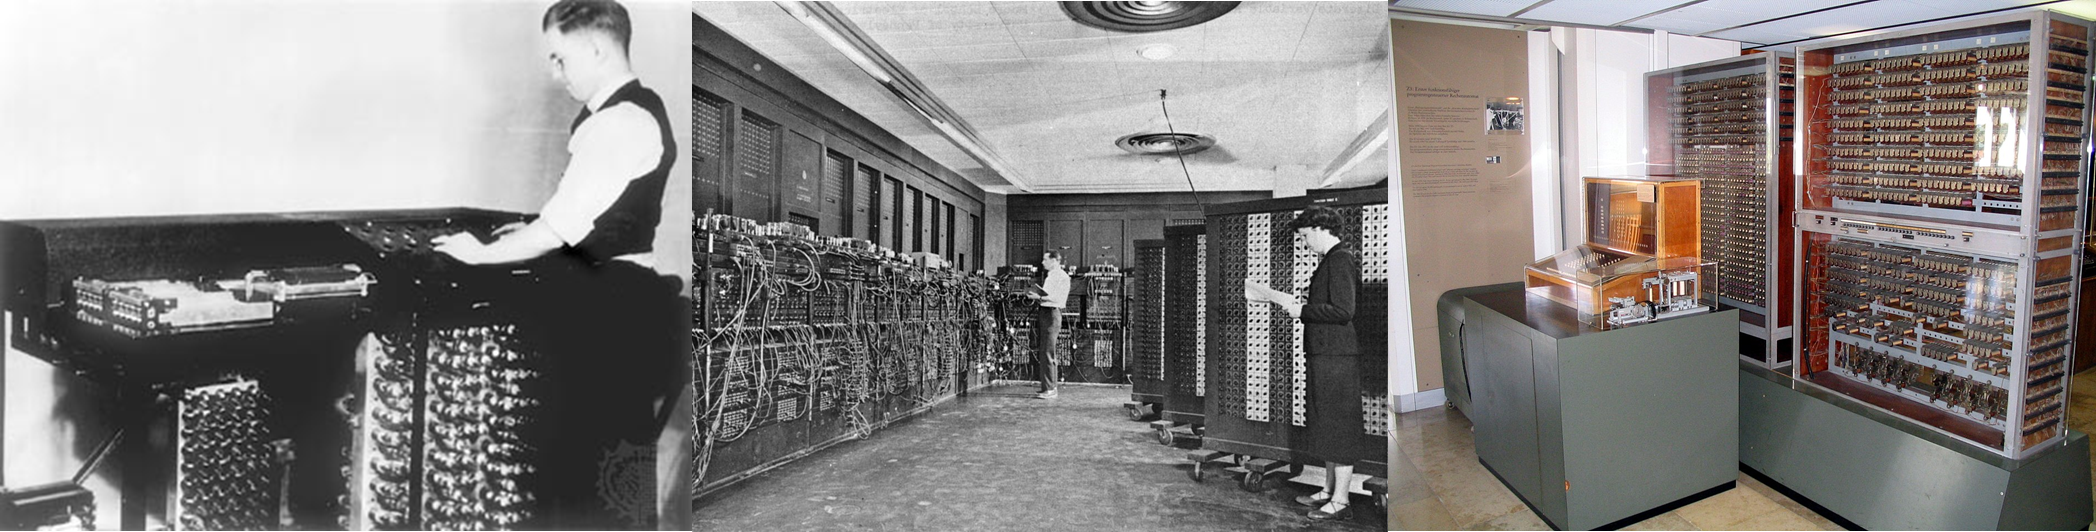
\includegraphics[width=1\linewidth]{images/historia/berry_eniac_z3} 

}

\caption{De izquierda a derecha: las computadoras ABC, ENIAC y Z3}\label{fig:berry}
\end{figure}

Este nuevo paradigma cambió la historia de la computación, como también lo hizo la invención del \emph{transistor} en 1947 en los Laboratorios Bell. Un \emph{transistor} es un dispositivo electrónico semiconductor que entrega una señal de salida en respuesta a una señal de entrada, mucho más pequeño que los tubos de vacío y que consumen menos energía eléctrica. Así, una computadora podía tener cientos de miles de transistores, no obstante ocupando mucho espacio.

Desde entonces, la computación ha evolucionado muy rápidamente, con la introducción de nuevos sistemas y conceptos, que llegan a los complejos y poderosos diseños electrónicos que caracterizan la vida actual. En un intento de caracterizar y resumir esta impactante evolución, algunos historiadores dividen al desarrollo de las computadoras modernas en ``generaciones'' (esta clasificación no es única y existen diversas versiones de la misma):

\begin{itemize}
\tightlist
\item
  \emph{Primera generación} (aprox. 1940-1958): se trata de las computadoras electrónicas que usaban tubos de vacío para su circuito interno. Los equipos eran enormes y ocupan habitaciones enteras. Consumían mucha electricidad y generaban demasiado calor. Podía llevar días o semanas modificar las conexiones para hacer que la computadora resuelva un problema diferente. Usaban tarjetas perforadas y cinta de papel para la lectura de datos e impresiones para mostrar las salidas.
\item
  \emph{Segunda generación} (aprox. 1958-1964): se caracteriza por el uso de \emph{transistores} (inventados en 1947) en lugar de tubos de vacío, permitiendo que las computadoras tengan un consumo eléctrico más eficiente, sean más baratas, más pequeñas y más rápidas.
\item
  \emph{Tercera generación} (aprox. 1964-1971): se inició en 1959 con el desarrollo de un circuito integrado (``chip'') que se trata de una pequeña placa de silicio sobre el cual se imprime un gran número de transistores conectados. La primera computadora de este estilo fue de IBM en 1960. Al ser más pequeñas y baratas, su uso llegó a una mayor audiencia. Se pudo interactuar con la máquina mediante teclados, monitores y un sistema operativo, que posibilitaba ejecutar múltiples acciones a la vez bajo el monitoreo de un programa central.
\item
  \emph{Cuarta generación} (aprox. 1971-presente): los avances tecnológicos permitieron construir la unidad entera de procesamiento de una computadora sobre un único chip de silicio (\emph{microprocesador}), incluyendo la memoria y los controles de entrada y salida de datos. Todo lo que en una computadora de la primera generación ocupaba una habitación entera, fue capaz de entrar en la palma de una mano. El primer microprocesador fue el Intel 4004 de 1971, mientras que la primera computadora de uso doméstico fue desarrollada por IBM en 1981. Surgieron también en esta generación el ratón (\emph{mouse}) y las interfaces gráficas de usuario (como Windows, en 1985).
\end{itemize}

\begin{figure}

{\centering 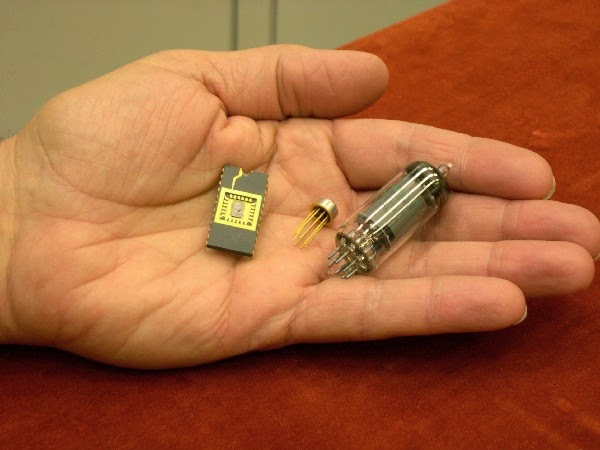
\includegraphics[width=0.5\linewidth]{images/historia/05_tubovacio_transistor_chip} 

}

\caption{De derecha a izquierda: un tubo de vacío, un transistor y un chip.}\label{fig:evolucion}
\end{figure}

\hypertarget{software-y-hardware}{%
\section{Software y hardware}\label{software-y-hardware}}

Como podemos ver, en la historia de la computación hubo dos aspectos que fueron evolucionando: las máquinas y los programas que las dirigen. Hacemos referencia a estos elementos como \emph{hardware} y \emph{software} respectivamente, y es la conjunción de ambos la que le da vida a la computación y hace posible la programación.

\begin{figure}

{\centering 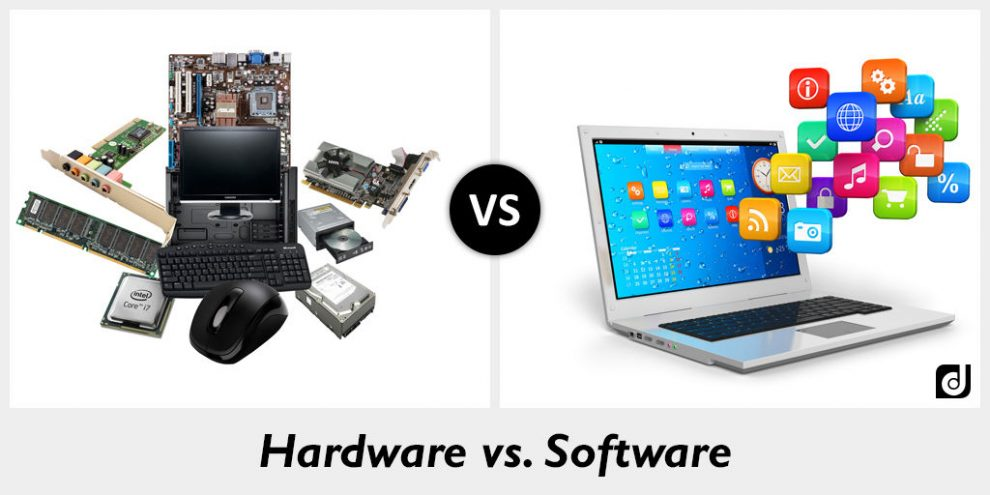
\includegraphics[width=0.5\linewidth]{images/intro/06_hardsoft} 

}

\caption{Representación de la diferencia entre hardware y software.}\label{fig:hardvssoft}
\end{figure}

El \emph{hardware} es el conjunto de piezas físicas y tangibles de la computadora. Existen diversas formas de clasificar a los elementos que componene al hardware, según distintos criterios:

\begin{table}[H]
\caption{Clasificación del hardware.}
%\begin{tabular}{@{}cccc@{}}
\begin{tabular}{ p{3.5cm} p{2.5cm} p{6cm}p{4cm}}
\toprule
Critero                               & Clasificación                       & Descripción                                                                                                                                                                                    & Ejemplos                                                                                                        \\ \midrule
\multirow{4}{*}{Según su utilidad}    & Dispositivos de procesamiento       & Son los que reciben las instrucciones mediante señales eléctricas y usan cálculos y lógica para interpretarlas y emitir otras señales eléctricas como resultado.                               & microprocesador, tarjeta gráfica, tarjeta de sonido, etc.                                                       \\ \cmidrule(l){2-4} 
                                      & Dispositivos de almacenamiento      & Son capaces de guardar información para que esté disponible para el sistema.                                                                                                                   & disco duro, pen drive, DVD, etc.                                                                                \\ \cmidrule(l){2-4} 
                                      & Dispositivos de entrada             & Captan instrucciones por parte de los usuarios y las transforman en señales eléctricas interpretables por la máquina.                                                                          & teclado, mouse, touch pad, etc.                                                                                 \\ \cmidrule(l){2-4} 
                                      & Dispositivos de salida              & Transforman los resultados de los dispositivos de procesamiento para presentarlos de una forma fácilmente interpretable para el usuario.                                                       & monitor, impresora, etc                                                                                         \\ \midrule
\multirow{2}{*}{Según su ubicación}   & Dispositivos internos               & Generalmente se incluye dentro de la carcasa de la computadora.                                                                                                                                & microprocesador, disco rígido, ventiladores, módem, tarjeta gráfica, fuente de alimentación, puertos, etc.      \\ \cmidrule(l){2-4} 
                                      & Dispositivos externos o periféricos & No se incluye dentro de la carcasa de la computadora y está al alcance del usuario                                                                                                             & monitor, teclado, mouse, joystick, micrófono, impresora, escáner, pen drive, lectores de código de barras, etc. \\ \midrule
\multirow{2}{*}{Según su importancia} & Hardware principal                  & Dispositvos esenciales para el funcionamiento de la computadora                                                                                                                                & microprocesador, disco rígido, memoria RAM, fuente de alimentación, monitor, etc.                               \\ \cmidrule(l){2-4} 
                                      & Hardware complementario             & Aquellos elementos no indispensables (claramente, dependiendo del contexto, alguna pieza del hardware que en alguna situación podría considerarse complementaria, en otras resulta principal). &                                                                                                                 \\ \bottomrule
\end{tabular}
\end{table}

\(~\)

Por otro lado tenemos al \emph{software}, que es el conjunto de todos los programas (es decir, todas las instrucciones que recibe la computadora) que permiten que el hardware funcione y que se pueda concretar la ejecución de las tareas. No tiene una existencia física, sino que es intangible. El software se puede clasificar de la siguiente forma:

\begin{table}[H]
\caption{Clasificación del software.}
\begin{tabular}{ p{4cm} p{6cm} p{6cm}}
\toprule
Clasificación                            & Descripción                                                                                                                                                               & Ejemplos                                                                                                                                                                                                            \\ \midrule
Software de sistema o software base      & Son los programas informáticos que están escritos en lenguaje de bajo nivel como el de máquina o ensamblador y cuyas instrucciones controlan de forma directa el hardware & BIOS o UEFIs (sistemas que se encargan de operaciones básicas como el arranque del sistema, la configuración del hardware, etc), sistemas operativos (Linux, Windows, iOS, Android), controladores o *drivers*, etc. \\ \midrule
Software de aplicación o utilitario      & Son los programas o aplicaciones que usamos habitualmente para realizar alguna tarea específica.                                                                          & procesadores de texto como Word, reproductor de música, Whatsapp, Guaraní, navegadores web, juegos, etc.                                                                                                            \\ \midrule
Software de programación o de desarrollo & Son los programas y entornos que nos permiten desarrollar nuestras propias herramientas de software o nuevos programas. Aquí se incluyen los lenguajes de programación    & C++, Java, Python, R, etc.                                                                                                                                                                                          \\ \bottomrule
\end{tabular}
\end{table}

\hypertarget{problemas-algoritmos-y-lenguajes-de-programaciuxf3n}{%
\section{Problemas, algoritmos y lenguajes de programación}\label{problemas-algoritmos-y-lenguajes-de-programaciuxf3n}}

Mencionamos anteriormente que la \emph{programación} consistía en instruir a una computadora para que resuelva un problema y que la comunicación de esas instrucciones debe ser realizada de forma clara. Es por eso que, ante un problema que debe ser resuelto computacionalmente, el primer paso es pensar detalladamente cuál puede ser una forma de resolverlo, es decir, crear un \emph{algoritmo}. Un \emph{algoritmo} es una estrategia consistente de un conjunto ordenado de pasos que nos lleva a la solución de un problema o alcance de un objetivo. Luego, hay que traducir el algoritmo elegido al idioma de la computadora.

Entonces, podemos decir que la resolución computacional de un problema consiste de dos etapas básicas:

\begin{enumerate}
\def\labelenumi{\arabic{enumi}.}
\tightlist
\item
  \emph{Diseño algorítmico}: desarrollar un algoritmo, o elegir uno existente, que resuelva el problema.
\item
  \emph{Codificación}: expresar un algoritmo en un lenguaje de programación para que la computadora lo pueda interpretar y ejecutar.
\end{enumerate}

Al aprender sobre programación, comenzamos enfrentándonos a problemas simples para los cuales la primera etapa parece sencilla, mientras que la codificación se torna dificultosa ya que hay que aprender las reglas del lenguaje de programación. Sin embargo, mientras que con práctica rápidamente podemos ganar facilidad para la escritura de código, el diseño algorítmico se torna cada vez más desafiante al encarar problemas más complejos. Es por eso que haremos hincapié en el planteo y desarrollo de algoritmos como una etapa fundamental en la programación.

\hypertarget{el-diseuxf1o-algoruxedtmico}{%
\subsection{El diseño algorítmico}\label{el-diseuxf1o-algoruxedtmico}}

Cotidianamente, hacemos uso de algoritmos para llevar adelante casi todas las actividades que realizamos: preparar el desayuno, sacar a pasear la mascota, poner en la tele un servicio de \emph{streaming} para ver una película, etc. Cada una de estas tareas requiere llevar adelante algunas acciones de forma ordenada, aunque no hagamos un listado de las mismas y procedamos casi sin pensar.

Sin embargo, cuando estamos pensando la solución para un problema que va a resolver una computadora, debemos ser claros y concretos, para asegurarnos de que al seguir los pasos del algoritmo se llegue a la solución y para que quien tenga que codificarlo, nosotros mismos u otras personas, lo pueda entender sin problemas. Por eso, el primer paso es idear un algoritmo para su solución y expresarlo por escrito, por ejemplo, en español, pero adaptando el lenguaje humano a formas lógicas que se acerquen a las tareas que puede realizar una computadora. En programación, el lenguaje artificial e informal que usan los desarrolladores en la confección de algoritmos recibe el nombre de \emph{pseudocódigo}. Es la herramienta que utilizamos para describir los algoritmos mezclando el lenguaje común con instrucciones de programación. No es en sí mismo un lenguaje de programación, es decir, la computadora no es capaz de entenderlo, sino que el objetivo del mismo es que el programador se centre en la solución lógica y luego lo utilice como guía al escribir el programa.

El pseudocódigo, como cualquier otro lenguaje, está compuesto por:

\begin{itemize}
\tightlist
\item
  Un \emph{léxico}: conjunto de palabras o frases válidas para escribir las instrucciones.
\item
  Una \emph{sintaxis}: reglas que establecen cómo se pueden combinar las distintas partes.
\item
  Una \emph{semántica}: significado que se les da a las palabras o frases.
\end{itemize}

El pseudocódigo sigue una \emph{estructura secuencial}: define una acción o instrucción que sigue a otra en secuencia. Esta estructura puede representarse de la siguiente forma:

\begin{verbatim}
ALGORITMO: "Ejemplo"
COMENZAR
    Acción 1
    Acción 2
    ...
    Acción N
FIN
\end{verbatim}

Se comienza con un título que describa el problema que el algoritmo resuelve, seguido por la palabra \texttt{COMENZAR}. Luego se detallan las acciones o instrucciones a seguir y se concluye con la palabra \texttt{FIN}. Por ejemplo, si nuestro problema es poner en marcha un auto, el algoritmo para resolverlo puede ser expresado mediante el siguiente pseudocódigo:

\begin{verbatim}
ALGORITMO: "Arrancar el auto"
COMENZAR
    INSERTAR la llave de contacto
    UBICAR el cambio en punto muerto
    GIRAR la llave hasta la posición de arranque
    SI el motor arranca 
        ENTONCES
            DEJAR la llave en posición "encendido"
        SI NO
            LLAMAR al mecánico
    FINSI
FIN
\end{verbatim}

Es importante destacar la presencia de sangrías (\emph{sangrado}) en el ejemplo anterior, que facilitan la lectura.

Los algoritmos suelen ser representados también mediante \emph{diagramas de flujo}, como el que se muestra en la siguiente figura\footnote{En este curso no emplearemos diagramas de flujo}.

\begin{figure}

{\centering 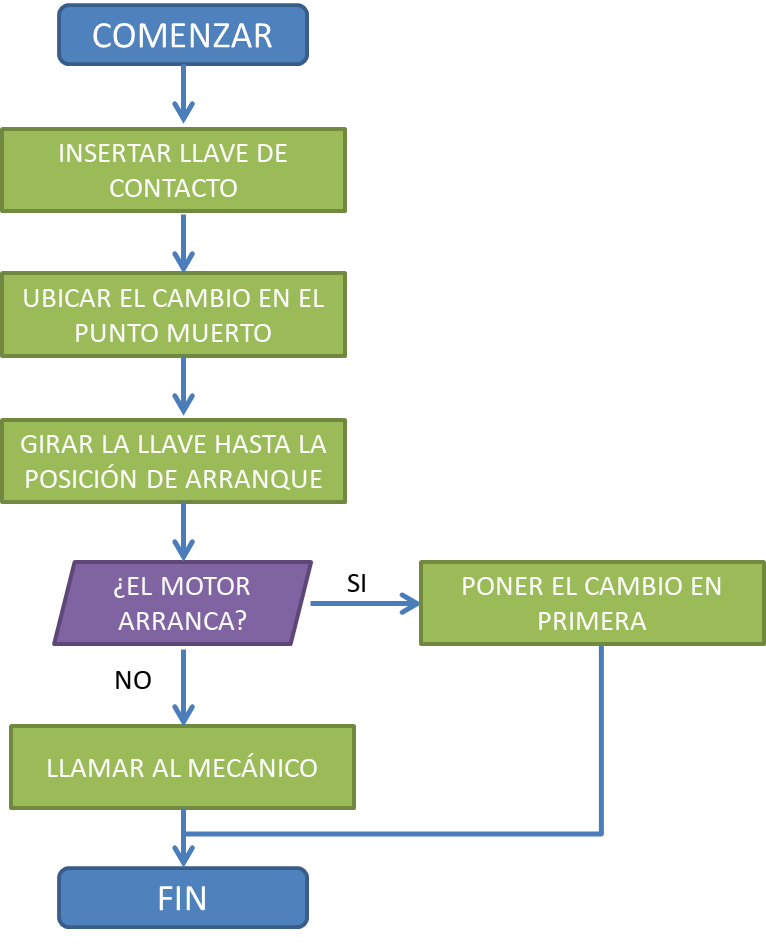
\includegraphics[width=0.7\linewidth]{images/intro/flujo} 

}

\caption{Ejemplo del algoritmo "Arrancar el auto" representado gráficamente con un diagrama de flujo.}\label{fig:algoritmo}
\end{figure}

\hypertarget{codificaciuxf3n}{%
\subsection{Codificación}\label{codificaciuxf3n}}

El algoritmo anterior está presentado en pseudocódigo utilizando el lenguaje español, una opción razonable para compartir esta estrategia entre personas que se comuniquen con este idioma. Claramente, si queremos presentarle nuestro algoritmo a alguien que sólo habla francés, el español ya no sería una buena elección, y mucho menos si queremos presentarle el algoritmo a una computadora. Para que una computadora pueda entender nuestro algoritmo, debemos traducirlo en un \emph{lenguaje de programación}, que, como dijimos antes, es un idioma artificial diseñado para expresar cómputos que puedan ser llevados a cabo por equipos electrónicos, es decir es un medio de comunicación entre el humano y la máquina.

Si bien hay distintos lenguajes de programación, una computadora en definitiva es un aparato que sólo sabe \emph{hablar} en \emph{binario}, es decir, sólo interpreta señales eléctricas con dos estados posibles, los cuales son representados por los dígitos binarios 0 y 1. Toda instrucción que recibe la computadora se construye mediante una adecuada y larga combinación de ceros y unos\footnote{Como vimos anteriormente, las computadoras de la primera generación no se manejaban con lenguajes de programación, sino que para introducir información e instrucciones en las primeras computadoras se usaban tarjetas perforadas, en las cuales los orificios representaban un ``0'' y las posiciones que no los tenían se entendían como un ``1'', de modo que la máquina podía operar empleando el sistema binario.}. Este sistema de código con ceros y unos que la computadora interpreta como instrucciones o conjuntos de datos se llama \emph{lenguaje de máquina} (o código de máquina).

Programar en lenguaje de máquina es muy complejo y lento, y es fácil cometer errores pero es difícil arreglarlos. Por eso a principios de la década de 1950 se inventaron los \emph{lenguaje ensambladores}, que usan palabras para representar simbólicamente las operaciones que debe realizar la computadora. Cada una de estas palabras reemplaza un código de máquina binario, siendo un poco más fácil programar. Imaginemos que deseamos crear un programa que permita sumar dos números elegidos por una persona. La computadora puede hacer esto si se lo comunicamos mediante un mensaje compuesto por una larga cadena de ceros y unos (lenguaje de máquina) que a simple vista no podríamos entender. Sin embargo, escrito en lenguaje de máquina, el programa se vería así (por ejemplo):

\begin{figure}

{\centering 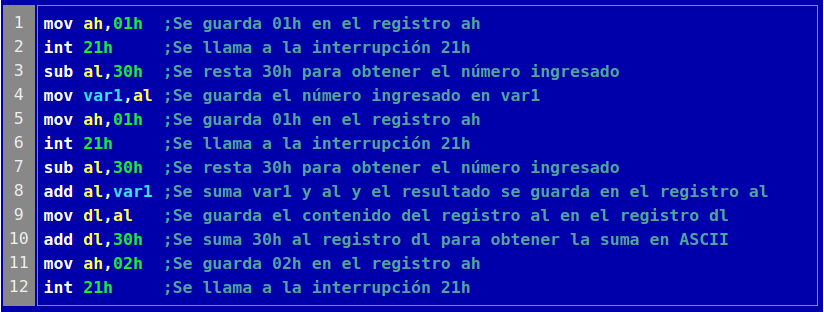
\includegraphics[width=1\linewidth]{images/intro/ensamblador} 

}

\caption{Programa en lenguaje ensamblador para leer dos números, sumarlos y mostrar el resultado. Al final de cada línea hay una descripción de la operación realizada.}\label{fig:unnamed-chunk-5}
\end{figure}

El programa que se encarga de traducir esto al código de máquina se llama \emph{ensamblador}. A pesar de que no haya ceros y unos como en el lenguaje de máquina, probablemente el código anterior tampoco sea fácil de entender. Aparecen instrucciones que tal vez podemos interpretar, como \emph{add} por sumar o \emph{sub} por substraer, pero está lleno de cálculos hexadecimales, referencias a posiciones en la memoria de la computadora y movimientos de valores que no lo hacen muy amigable. Por eso, a pesar de que la existencia de los lenguajes ensambladores simplificó mucho la comunicación con la computadora, se hizo necesario desarrollar lenguajes que sean aún más sencillos de usar.

Por ejemplo, con el lenguaje que vamos a aprender, R, el problema de pedirle dos números a una persona y sumarlos se resumen en las siguientes líneas de código:

\begin{verbatim}
n1 <- scan()
n2 <- scan()
print(n1 + n2)
\end{verbatim}

En las dos primeras líneas con la sentencia \texttt{scan()} (que quiere decir ``escanear'', ``leer'') se le pide a la persona que indique dos números y en la tercera línea se muestra el resultado de la suma, con la sentencia \texttt{print()} (``imprimir'', ``mostrar''). Mucho más corto y entendible.

Esta simplificación es posible porque nos permitimos \emph{ignorar} ciertos aspectos del proceso que realiza la computadora. Todas esas acciones que se ven ejemplificadas en la imagen con el código ensamblador se llevan a cabo de todas formas, pero no lo vemos. Nosotros sólo tenemos que aprender esas últimas tres líneas de código, de forma que nos podemos concentrar en el problema a resolver (ingresar dos números, sumarlos y mostrar el resultado) y no en las complejas operaciones internas que tiene que hacer el microprocesador.

En programación, la idea de simplificar un proceso complejo ignorando algunas de sus partes para comprender mejor lo que hay que realizar y así resolver un problema se conoce como \emph{abstracción}\footnote{La abstracción no es una idea exclusiva de la programación. Se encuentra, también, por ejemplo, en el \emph{arte abstracto}.}. Esto quiere decir que los lenguajes de programación pueden tener distintos niveles de abstracción:

\begin{itemize}
\tightlist
\item
  \emph{Lenguajes de bajo nivel de abstracción}: permiten controlar directamente el \emph{hardware} de la computadora, son específicos para cada tipo de máquina, y son más rígidos y complicados de entender para nosotros. El lenguaje ensamblador entra en esta categoría.
\item
  \emph{Lenguajes de alto nivel de abstracción}: diseñados para que sea fácil para los humanos expresar los algoritmos sin necesidad de entender en detalle cómo hace exactamente el hardware para ejecutarlos. El lenguaje que utilizaremos en este taller, R, es de alto nivel. Son independientes del tipo de máquina.
\item
  \emph{Lenguajes de nivel medio de abstracción}: son lenguajes con características mixtas entre ambos grupos anteriores.
\end{itemize}

\begin{figure}

{\centering 
\includegraphics[width=0.7\linewidth]{images/intro/07_lenguajes} 

}

\caption{Distintos lenguajes de programación y sus logos.}\label{fig:lenguajes}
\end{figure}

Si bien podemos programar usando un lenguaje de alto nivel para que nos resulte más sencillo, \emph{alguien} o \emph{algo} debe traducirlo a lenguaje de máquina para que la computadora, que sólo entiende de ceros y unos, pueda realizar las tareas. Esto también es necesario incluso si programáramos en lenguaje ensamblador. Para estos procesos de traducción se crearon los \emph{compiladores} e \emph{intérpretes}.

Un \emph{compilador} es un programa que toma el código escrito en un lenguaje de alto nivel y lo traduce a código de máquina, guardándolo en un archivo que la computadora ejecutará posteriormente (archivo ejecutable). Para ilustrar el rol del compilador, imaginemos que alguien que sólo habla español le quiere mandar una carta escrita en español a alguien que vive en Alemania y sólo habla alemán. Cuando esta persona la reciba, no la va a entender. Se necesita de un intermediario que tome la carta en español, la traduzca y la escriba en alemán y luego se la mande al destinatario, quien ahora sí la podrá entender. Ese es el rol de un \emph{compilador} en la computadora. Ahora bien, el resultado de la traducción, que es la carta escrita en alemán, sólo sive para gente que hable alemán. Si se quiere enviar el mismo mensaje a personas que hablen otros idiomas, necesitaremos hacer la traducción que corresponda. De la misma forma, el código generado por un compilador es específico para cada máquina, depende de su arquitectura.

Además de los compiladores, para realizar este pasaje también existen los \emph{intérpretes}. Un intérprete es un programa que traduce el código escrito en lenguaje de alto nivel a código de máquina, pero lo va haciendo a medida que se necesita, es decir, su resultado reside en la memoria temporal de la computadora y no se genera ningún archivo ejecutable. Siguiendo con el ejemplo anterior, es similar a viajar a Alemania con un intérprete que nos vaya traduciendo en vivo y en directo cada vez que le queramos decir algo a alguien de ese país. En su implementación por defecto, el lenguaje R es interpretado, no compilado.

Concluyendo, gracias al concepto de la \emph{abstracción} podemos escribir programas en un lenguaje que nos resulte fácil entender, y gracias al trabajo de los \emph{compiladores} e \emph{intérpretes} la computadora podrá llevar adelante las tareas necesarias.

Cada una de las acciones que componen al algoritmo son codificadas con una o varias \emph{instrucciones} o \emph{sentencias}, expresadas en el lenguaje de programación elegido, y el conjunto de todas ellas constituye un \emph{programa}. El programa se guarda en un \emph{archivo} con un nombre generalmente dividido en dos partes por un punto, por ejemplo: \texttt{mi\_primer\_programa.R}. La primera parte es la \emph{raíz} del nombre con la cual podemos describir el contenido del archivo. La segunda parte es indicativa del uso del archivo, por ejemplo, \texttt{.R} indica que contiene un programa escrito en el lenguaje R. El proceso general de ingresar o modificar el contenido de un archivo se denomina \emph{edición}.

\hypertarget{errores-de-programaciuxf3n}{%
\section{Errores de programación}\label{errores-de-programaciuxf3n}}

Apenas iniciemos nuestro camino en el mundo de la programación nos daremos cuenta que tendremos siempre ciertos compañeros de viaje: los \emph{errores}. Muchas veces nos pasará que queremos ejecutar nuestro código y el mismo no anda o no produce el resultado esperado. No importa cuán cuidadosos seamos, ni cuánta experiencia tengamos, los errores están siempre presentes. Con el tiempo y práctica, vamos a poder identificarlos y corregirlos con mayor facilidad, pero probablemente nunca dejemos de cometerlos.

A los errores en programación se los suele llamar \emph{bugs} (insecto o bicho en inglés) y el proceso de la corrección de los mismos se conoce como \emph{debugging} (depuración)\footnote{Algunos usan el término bug para referirse exclusivamente a errores lógicos}. Se dice que esta terminología proviene de 1947, cuando una computadora en la Universidad de Harvard (la \emph{Mark II}) dejó de funcionar y finalmente se descubrió que la causa del problema era la presencia de una polilla en un relé electromagnético de la máquina. Sin embargo, otros historiadores sostienen que el término ya se usaba desde antes.

\begin{figure}

{\centering 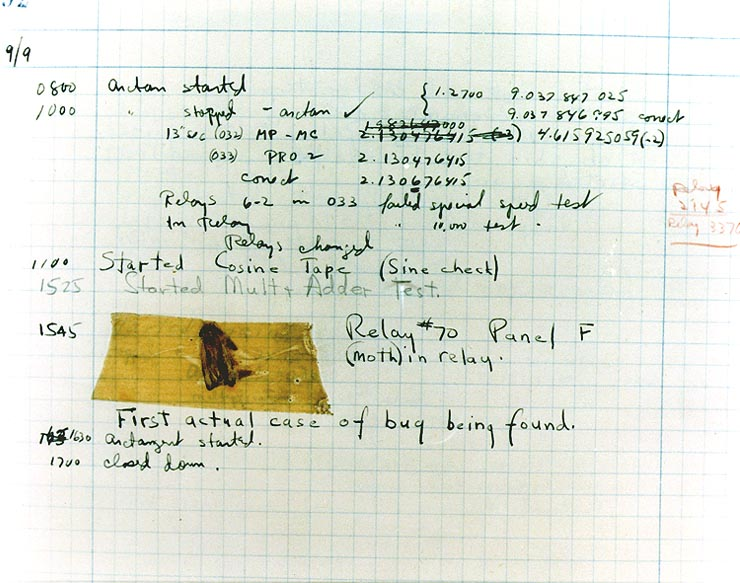
\includegraphics[width=0.7\linewidth]{images/intro/First_Computer_Bug} 

}

\caption{La polilla (bug) encontrada por la científica de la computación Grace Hooper en la Mark II fue pegada con cinta en un reporte sobre el malfuncionamiento de la máquina.}\label{fig:unnamed-chunk-6}
\end{figure}

A continuación se presenta una de las posibles clasificaciones de los errores que se pueden cometer en programación:

\begin{itemize}
\item
  \emph{Errores de sintaxis}. Tal como el lenguaje humano, los lenguajes de programación tienen su propio vocabulario y su propia sintaxis, que es el conjunto de reglas gramaticales que establecen cómo se pueden combinar las distintas partes. Estas reglas sintácticas determinan que ciertas sentencias están correctamente construidas, mientras que otras no. Cuando ejecutamos un programa, el compilador o el intérprete chequea si el mismo es sintácticamente correcto. Si hemos violado alguna regla, por ejemplo, nos faltó una coma o nos sobra un paréntesis, mostrará un mensaje de error y debemos editar nuestro programa para corregirlo. En estos casos, hay que interpretar el mensaje de error, revisar el código y corregir el error.
\item
  \emph{Errores lógicos}. Se presentan cuando el programa puede ser compilado sin errores pero arroja resultados incorrectos o ningún resultado. El software no muestra mensajes de error, debido a que, por supuesto, no sabe cuál es el resultado deseado, sino que sólo se limita a hacer lo que hemos programado. En estos casos hay que revisar el programa para encontrar algún error en su lógica. Este tipo de errores suelen ser los más problemáticos. Algunas ideas para enfrentarlos incluyen volver a pensar paso por paso lo que se debería hacer para solucionar el problema y compararlo con lo que se ha programado, agregar pasos para mostrar resultados intermedios o emplear herramientas especializadas de \emph{debugging} (llamadas \emph{debugger}) para explorar el código paso a paso hasta identificar el error.
\item
  \emph{Errores en la ejecución} (\emph{runtime errors}). Se presentan cuando el programa está bien escrito, sin errores lógicos ni sintácticos, pero igualmente se comporta de alguna forma incorrecta. Se dan a pesar de que el programa ande bien en el entorno de desarrollo del programador, pero no cuando algún usuario lo utiliza en algún contexto particular. Puede ser que se intente abrir un archivo que no existe, que el proceso supere la memoria disponible, que tomen lugar operaciones aritméticas no definidas como la división por cero, etc.
\end{itemize}

Los errores en la programación son tan comunes, que un científico de la computación muy reconocido, Edsger Dijkstra, dijo una vez: ``si la depuración es el proceso de eliminar errores, entonces la programación es el proceso de generarlos''. Ante la presencia de uno, no hay más que respirar profundo y con paciencia revisar hasta encontrarlo y solucionarlo.

\begin{figure}

{\centering 
\includegraphics[width=0.5\linewidth]{images/intro/08_bug} 

}

\caption{Encontrando un bug en un programa.}\label{fig:bug}
\end{figure}

\hypertarget{procesador-ambiente-y-acciones}{%
\section{Procesador, ambiente y acciones}\label{procesador-ambiente-y-acciones}}

Hemos definido a un algoritmo como una lista de instrucciones para resolver un problema. En este contexto, se entiende por \emph{procesador} a todo agente capaz de comprender los pasos de un algoritmo y ejecutar el trabajo indicado por el mismo. Para cumplir con el objetivo, el procesador emplea ciertos recursos que tiene a disposición. Todos los elementos disponibles para ser utilizados por el procesador constituyen su \emph{entorno} o \emph{ambiente}. Cada una de las instrucciones que componen el algoritmo modifican el entorno de alguna manera y se denominan \emph{acciones}.

Ejemplificaremos estos conceptos con los siguientes ejemplos:

\emph{Ejemplo 1}

\begin{itemize}
\tightlist
\item
  \emph{Problema}: preparar una tortilla de 6 huevos.
\item
  \emph{Entorno}: una mesa, una hornalla, una sartén, un plato, un tenedor, aceite, una fuente con huevos, un tarro de basura.
\item
  \emph{Procesador}: una persona adulta.
\item
  \emph{Acciones comprensibles por el procesador}: agarrar un huevo, romper un huevo en un plato, batir huevos, poner aceite, poner en la sartén, poner al fuego, retirar del fuego, tirar las cáscaras, encender el fuego.
\end{itemize}

¿Cuál es un algoritmo adecuado para solucionar este problema? Podría ser:

\begin{verbatim}
ALGORITMO: "Preparar una tortilla de 6 huevos"
COMENZAR
    ROMPER seis huevos en un plato
    TIRAR las cáscaras en el tacho
    BATIR los huevos
    CALENTAR aceite en la sartén
    PONER el contenido del plato en la sartén
    ESPERAR diez minutos
    RETIRAR la tortilla del fuego
    APAGAR el fuego
FIN
\end{verbatim}

\emph{Ejemplo 2}

\begin{itemize}
\tightlist
\item
  \emph{Problema}: calcular el factorial del número 5.
\item
  \emph{Entorno}: se dispone de una calculadora común.
\item
  \emph{Procesador}: una persona adulta.
\item
  \emph{Acciones comprensibles por el procesador}: pulsar teclas de la calculadora.
\end{itemize}

¿Cuál es un algoritmo adecuado para solucionar este problema? Podría ser:

\begin{verbatim}
ALGORITMO: "Calcular 5!"
COMENZAR
    PULSAR [ON]
    PULSAR [1]
    PULSAR [X]
    PULSAR [2]
    PULSAR [X]
    PULSAR [3]
    PULSAR [X]
    PULSAR [4]
    PULSAR [X]
    PULSAR [5]
    PULSAR [=]
    MOSTRAR la pantalla
FIN
\end{verbatim}

Las acciones del algoritmo pueden clasificarse en función de su complejidad:

\begin{itemize}
\tightlist
\item
  \emph{Acción primitiva}: acción sencilla directamente realizable por el procesador sin necesidad de contar con mayor información.
\item
  \emph{Acción compuesta}: acción integrada por una sucesión de acciones primitivas.
\end{itemize}

La descripción de un algoritmo en términos de acciones compuestas puede facilitar su comprensión, pero al desarrollar el programa será necesario descomponerlas en acciones primitivas que son las que realmente ejecuta el procesador. Por ejemplo, la acción compuesta en el ejemplo de la tortilla de ``romper seis huevos en un plato'' puede descomponerse en acciones más simples:

\begin{verbatim}
REPETIR 6 VECES
    TOMAR un huevo
    GOLPEAR el huevo para generar una fractura en la cáscara
    EJERCER presión sobre la cáscara
    DERRAMAR la clara y la yema sobre el plato
\end{verbatim}

En el contexto de la resolución de un problema computacional, el \emph{procesador} será la computadora; las acciones estarán dadas por las sentencias disponibles en el lenguaje de programación utilizado o las que podamos crear en base al mismo; y el \emph{ambiente} estará constituido por un conjunto de variables, estructuras de datos, funciones y otros elementos que serán de utilidad en la programación.

\hypertarget{r-y-rstudio}{%
\section{R y RStudio}\label{r-y-rstudio}}

Como dijimos anteriormente, pondremos en práctica los conceptos sobre programación utilizando \textbf{R}, un lenguaje orientado a la realización de procesos estadísticos y gráficos. A diferencia de muchos otros, este es un software libre y gratuito: se distribuye bajo la licencia \emph{GNU GPLv2} que establece la libertad de usarlo con cualquier propósito, de ver cómo fue hecho, cómo funciona y modificarlo, de distribuir copias y crear contribuciones y agregados para que estén disponibles para otros \footnote{\textbf{R} tiene una comunidad de usuarios muy activa, de las más diversas áreas, con muchos blogs, portales y encuentros en persona para buscar y recibir ayuda. Por ejemplo, existe el grupo de R en Rosario: (\url{https://renrosario.rbind.io})}.

Si bien R será nuestro medio de comunicación con la computadora, vamos a usar otro programa que brinda algunas herramientas para facilitar nuestro trabajo de programación, es decir, vamos a usar un \textbf{entorno de desarrollo integrado} (o \emph{IDE}, por \emph{integrated development environment}). Un IDE es un programa que hace que la codificación sea más sencilla porque permite manejar varios archivos de código, visualizar el \emph{ambiente} de trabajo, utilizar resaltado con colores para distintas partes del código, emplear autocompletado para escribir más rápido, explorar páginas de ayuda, implementar estrategias de depuración e incluso intercalar la ejecución de sentencias con la visualización de los resultados mientras avanzamos en el análisis o solución del problema. El IDE más popularmente empleado para programar con R es \textbf{RStudio} y será el programa que estaremos usando todo el tiempo.

Para instalar estos programas, se debe visitar las páginas oficiales de \href{https://www.r-project.org/}{R} y de \href{https://www.rstudio.org/}{RStudio}, descargar los instaladores y ejecutarlos. En este \href{https://www.youtube.com/watch?v=D9Bp11iZssc}{enlace} se presenta un video con la instalación completa.

\hypertarget{organizaciuxf3n-de-rstudio}{%
\subsection{Organización de RStudio}\label{organizaciuxf3n-de-rstudio}}

Cuando se abre RStudio se pueden visualizar cuatro paneles:

\begin{figure}

{\centering 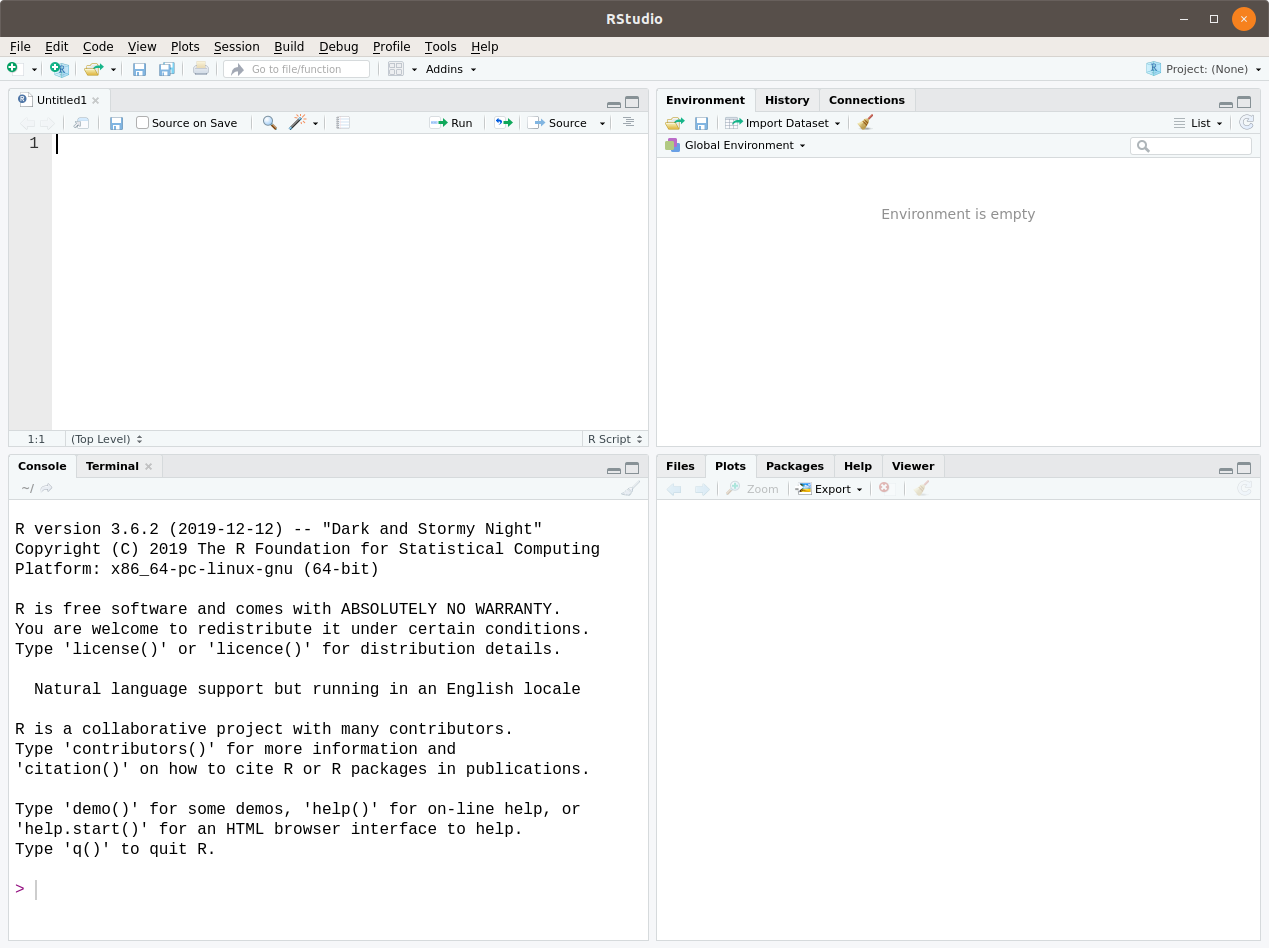
\includegraphics[width=1\linewidth]{images/intro/12_AbrirRStudio} 

}

\caption{Captura de pantalla de RStudio}\label{fig:unnamed-chunk-10}
\end{figure}

\begin{itemize}
\item
  A la izquierda:

  \begin{itemize}
  \tightlist
  \item
    Arriba está el \textbf{editor de archivos}. Es el lugar donde escribiremos y editaremos nuestros programas, para luego guardarlos (una especie de Bloc de Notas* o de un \emph{Word} muy simple). La primera vez que se abre RStudio después de su instalación puede ser que este panel no esté presente, pero aparece si vamos a \texttt{File\ \textgreater{}\ New\ File\ \textgreater{}\ R\ Script}, con el atajo \texttt{Ctrl\ +\ Shift\ +\ N} o haciendo clic en el primer ícono de la barra de herramientas. Podemos abrir varios archivos a la vez.
  \item
    Abajo está la \textbf{consola}. Es la ventana que se comunica con R. A través de ella se envían las instrucciones o \emph{sentencias} a R para que las evalúe (también decimos, que las ejecute o corra) y se visualizan los resultados.
  \end{itemize}
\item
  Arriba a la derecha hay un panel con algunas pestañas:

  \begin{itemize}
  \tightlist
  \item
    \textbf{Environment} (\emph{ambiente}): muestra todos los elementos que componen al ambiente o entorno.
  \item
    \textbf{History} (\emph{historial}): lista todas las instrucciones que R ha corrido anteriormente.
  \item
    \textbf{Otras más que no nos interesan por ahora}
  \end{itemize}
\item
  Abajo a la derecha hay otro panel con más pestañas:

  \begin{itemize}
  \tightlist
  \item
    \textbf{Files}: explorador de archivos de la computadora
  \item
    \textbf{Plots}: ventana donde aparecen los gráficos si es que nuestro código produce alguno
  \item
    \textbf{Packages}: listado de los ``paquetes'' que tenemos instalados (ver más adelante)
  \item
    \textbf{Help}: manual de ayuda sobre todas las funciones de R
  \item
    \textbf{Viewer}: espacio para ver salidas de los programas con algún componente dinámico o interactivo.
  \end{itemize}
\end{itemize}

\hypertarget{uso-de-rstudio}{%
\subsection{Uso de RStudio}\label{uso-de-rstudio}}

Podemos usar la consola de R que encontramos en el panel de la izquierda para introducir allí nuestras sentencias y al hacer \texttt{Enter} serán evaluadas, produciendo algún resultado. Por ejemplo, podemos hacer algunos cálculos matemáticos como dividir, multiplicar, sumar, restar, calcular potencias, logaritmos, raíces y mucho más:

\begin{Shaded}
\begin{Highlighting}[]
\DecValTok{1} \SpecialCharTok{+} \DecValTok{2}
\end{Highlighting}
\end{Shaded}

\begin{verbatim}
[1] 3
\end{verbatim}

\begin{Shaded}
\begin{Highlighting}[]
\DecValTok{5} \SpecialCharTok{*} \DecValTok{3}
\end{Highlighting}
\end{Shaded}

\begin{verbatim}
[1] 15
\end{verbatim}

\begin{Shaded}
\begin{Highlighting}[]
\FunctionTok{exp}\NormalTok{(}\DecValTok{2}\NormalTok{)}
\end{Highlighting}
\end{Shaded}

\begin{verbatim}
[1] 7.389056
\end{verbatim}

\begin{Shaded}
\begin{Highlighting}[]
\FunctionTok{sqrt}\NormalTok{(}\DecValTok{100}\NormalTok{)}
\end{Highlighting}
\end{Shaded}

\begin{verbatim}
[1] 10
\end{verbatim}

\begin{Shaded}
\begin{Highlighting}[]
\DecValTok{1} \SpecialCharTok{/} \DecValTok{0}
\end{Highlighting}
\end{Shaded}

\begin{verbatim}
[1] Inf
\end{verbatim}

\begin{Shaded}
\begin{Highlighting}[]
\NormalTok{(}\DecValTok{2} \SpecialCharTok{+}\NormalTok{ 3i) }\SpecialCharTok{*}\NormalTok{ (}\DecValTok{3} \SpecialCharTok{+}\NormalTok{ 6i)}
\end{Highlighting}
\end{Shaded}

\begin{verbatim}
[1] -12+21i
\end{verbatim}

\begin{Shaded}
\begin{Highlighting}[]
\NormalTok{1i }\SpecialCharTok{\^{}} \DecValTok{2}
\end{Highlighting}
\end{Shaded}

\begin{verbatim}
[1] -1+0i
\end{verbatim}

Si bien podemos escribir nuestras sentencias en la consola y dar \texttt{Enter} para que se ejecuten, en general queremos que queden escritas y guardadas en el archivo de código, por eso vamos a escribir nuestros programas en el panel de arriba a la izquierda. Una vez que escribimos una sentencia en el script, podemos \emph{correrla} (es decir, enviarla a la consola para que se ejecute) haciendo clic en el ícono \emph{Run} o con el atajo \emph{Ctrl + Enter}. De esta forma, se \emph{corre} la línea en la cual está el cursor o las líneas que hayamos seleccionado.

En todo lenguaje de programación existe un caracter especial que, al ser colocado al comienzo de una línea de código, le indica al software que dicha línea no debe ser evaluada. Esto se utiliza para incluir \textbf{comentarios}, es decir, líneas que expresan en español explicaciones o aclaraciones para nosotros mismos u otros que puedan utilizar nuestro código. También se utiliza para añadir encabezados con descripciones sobre el script, o indicar distintas secciones o partes en el programa. En R, este caracter especial es el símbolo numera (\texttt{\#}). Si \emph{corremos} líneas que empiezan con \texttt{\#}, R no hará nada con ellas, las salteará. Por ejemplo

\begin{Shaded}
\begin{Highlighting}[]
\DecValTok{5}\SpecialCharTok{\^{}}\DecValTok{1}
\end{Highlighting}
\end{Shaded}

\begin{verbatim}
[1] 5
\end{verbatim}

\begin{Shaded}
\begin{Highlighting}[]
\CommentTok{\# 5\^{}2}
\DecValTok{5}\SpecialCharTok{\^{}}\DecValTok{3}
\end{Highlighting}
\end{Shaded}

\begin{verbatim}
[1] 125
\end{verbatim}

\hypertarget{diseuxf1o-del-sistema-r}{%
\subsection{Diseño del sistema R}\label{diseuxf1o-del-sistema-r}}

R Se divide en dos partes:

\begin{itemize}
\item
  La \textbf{base} (\emph{R Base}), que se instala cuando descargamos el programa desde \href{https://cran.r-project.org/}{CRAN} (``Comprehensive R Archive Network''). Contiene, entre otras cosas, una serie de herramientas básicas y fundamentales de R.
\item
  \textbf{Paquetes adicionales}. Un paquete es un conjunto de archivos que se descarga de forma opcional desde CRAN u otros repositorios y que sirven para hacer alguna tarea especial. Por ejemplo, para poder hacer gráficos lindos, se puede usar un paquete que se llama \texttt{ggplot2}.
\end{itemize}

Como dijimos antes, en la pestaña \emph{Packages} del panel de abajo a la derecha tiene el listado de todos los paquetes que ya están instalados (muchos vienen con R Base). Allí también hay un botón para instalar nuevos, aunque otra opción es correr la sentencia \texttt{install.packages("nombredelpaquete")}, por ejemplo, \texttt{install.packages("ggplot2")}. Un paquete se instala una sola vez, pero cada vez que lo queramos usar debemos \emph{cargarlo} para que las herramientas que trae queden a nuestra disposición. Eso se hace con la sentencia \texttt{library("nombredelpaquete")}, por ejemplo, \texttt{library("ggplot2")}.

\hypertarget{guuxeda-de-estilo}{%
\section{Guía de estilo}\label{guuxeda-de-estilo}}

Es sumamente importante mantener la prolijidad en la escritura tanto del pseudocódigo como de los programas, para facilitar la lectura de los mismos, especialmente cuando estamos trabajando con problemas largos. Siempre hay que tener en cuenta de que cuando escribimos un programa, tenemos dos públicos potenciales: integrantes de nuestro equipo de trabajo que tienen leer el código y hacer sus propios aportes y nosotros mismos en el futuro, cuando retomemos código hecho en el pasado y necesitemos interpretar qué es lo que hicimos hacer.

Es por eso que se establecen conjuntos de reglas para controlar y unificar la forma de escribir programas, que se conocen como \textbf{guía de estilo}. Estas reglas cubren aspectos como, por ejemplo, la forma de escribir comentarios en el código, la utilización de espacios o renglones en blanco, el formato de los nombres para los elementos que creamos nosotros mismos (como las funciones) y para los archivos que generamos, etc. Una \emph{guía de estilo} no indica la única forma de escribir código, ni siquiera la forma correcta de hacerlo, sino que establece una convención para que todos trabajen de la misma forma, basándose en costumbres que sí se ha visto que pueden tener más ventajas que otras.

Por ejemplo, para programar en R, existe una guía de estilo llamada \href{https://style.tidyverse.org/}{The tidyverse style guide}, que es la que utilizan la gente de Google y de RStudio. En este curso vamos a adherir a sus recomendaciones. Si bien es una lectura muy interesante, particularmente si tenés intenciones de profundizar tus conocimientos sobre programación en R, no es necesario que lean dicha guía completa. Por ahora es suficiente con que imiten con atención el estilo que usamos en los ejemplos provistos en esta guía.

Recordemos siempre que seguir un buen estilo para programar es como hacer uso de una correcta puntuación cuando escribimos, podemos entendernos sin ella, peroesmuchomasdificilleerloqueescribimossinolarespetamosno?

\hypertarget{objetos-y-operadores}{%
\chapter{Objetos y operadores}\label{objetos-y-operadores}}

Hemos mencionado que para resolver un problema computacional se necesita de un \emph{procesador}, capaz de entender y ejecutar ciertas \emph{acciones} a partir de ciertos elementos disponibles en el \emph{ambiente} o \emph{entorno}. En este capítulo vamos aprender acerca de dichos elementos, a los que llamamos \emph{objetos}.

\hypertarget{objetos}{%
\section{Objetos}\label{objetos}}

Los \textbf{objetos} son las distintas piezas de información, o más sencillamente, \emph{datos}, que componen al \emph{entorno} y que el procesador debe manipular para resolver una tarea. Las distintas acciones del algoritmo van creando o modificando a los objetos del entorno. A medida que avancemos, veremos que hay distintas clases de objetos, algunos con estructuras más simples y otros más complejos. Es más, cada lenguaje de programación propone su propio catálogo de clases de objetos y cada programador puede crear otras nuevas. Sin embargo, en general todos los lenguajes tienen en común el hecho de que sus objetos pueden almacenar los siguientes tres tipos de datos básicos, conocidos como \textbf{tipos de datos primitivos}:

\begin{itemize}
\tightlist
\item
  \textbf{Datos de tipo numérico}: representan valores escalares de forma numérica y permiten realizar operaciones aritméticas comunes. Ejemplo: 230, 2.
\item
  \textbf{Datos de tipo caracter}: representan texto y no es posible hacer operaciones matemáticas con ellos. Representamos estos valores entre comillas. Ejemplo: ``hola'', ``chau123''
\item
  \textbf{Datos de tipo lógico}: pueden tomar dos valores (\emph{VERDADERO} o \emph{FALSO}), ya que representan el resultado de alguna comparación entre otros objetos. En R, estos valores son \texttt{TRUE} y \texttt{FALSE}, escritos sin comillas.
\end{itemize}

De manera general, al nombre de un objeto se le dice \textbf{identificador}, el cual es una secuencia de caracteres alfanuméricos que sirve para identificarlo a lo largo del algoritmo. Nombrar los objetos hace posible referirse a los mismos. La elección de los identificadores es una tarea del programador, pero cada lenguaje tiene sus propias reglas. Por ejemplo, en R los nombres de los objetos:

\begin{itemize}
\tightlist
\item
  Deben empezar con una letra o un punto (no pueden empezar con un número).
\item
  Sólo pueden contener letras, números, guiones bajos y puntos (se puede forzar a R para que acepte nombres con otros caracteres, pero no es aconsejable).
\item
  No se pueden usar las siguientes palabras como nombres, ya que son palabras claves reservadas para R: \texttt{break}, \texttt{else}, \texttt{FALSE}, \texttt{for}, \texttt{function}, \texttt{if}, \texttt{Inf}, \texttt{NA}, \texttt{NaN}, \texttt{next}, \texttt{repeat}, \texttt{return}, \texttt{TRUE}, \texttt{while}.
\end{itemize}

Es aconsejable elegir un nombre que sea representativo de la información que va a guardar el objeto, ya que esto facilita la lectura y la comprensión tanto del algoritmo como del programa. Por ejemplo, si se necesita un objeto para guardar el valor numérico del precio de algún producto, el identificador \texttt{p} sería una mala elección, mientras que \texttt{precio} sería mejor. Si se necesitan varios identificadores para distinguir los precios de diversos productos, podríamos usar algo como \texttt{precio\_manzana}, \texttt{precio\_banana}, etc. Otra opción podría ser \texttt{preciomanzana} o \texttt{precioManzana}, pero en este curso seguiremos la convención de usar guiones bajos para facilitar la lectura de los nombres elegidos. No sería posible usar como identificador a \texttt{precio\ manazana}, puesto que un nombre no puede tener espacios.

Ciertos objetos almacenan temporalmente un valor durante la ejecución de un proceso y su contenido puede cambiar mientras corre el programa. Este tipo de objetos reciben el nombre de \textbf{variables}. Por ejemplo, en un programa creado para un comercio puede existir un objeto llamado \texttt{stock} (identificador) de tipo numérico que representa la cantidad de artículos disponibles y cuyo valor se modifica cada vez que se registra una nueva venta. Podemos pensar a una variable como una caja etiquetada con un nombre (su identificador) y que guarda un valor (numérico, lógico o de caracter).

\begin{figure}

{\centering 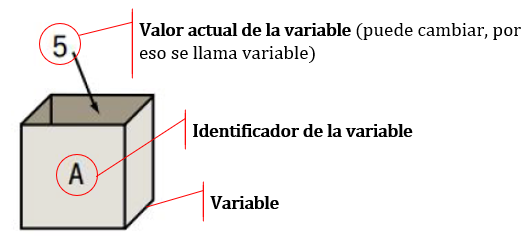
\includegraphics[width=0.5\linewidth]{images/02_obj/09_cajas2} 

}

\caption{La variable A contiene al valor 5.}\label{fig:cajas}
\end{figure}

Si un objeto tiene siempre necesariamente un valor fijo, se dice que es una \textbf{constante}. El valor es siempre el mismo para cualquier ejecución del programa, es decir, no puede cambiar de una ejecución a otra. Son ejemplos de constantes el número de meses del año, las constantes matemáticas tales como el número \(\pi\), los factores de conversión de unidades de medida, etc. Las constantes pueden usarse literalmente, es decir, usando explícitamente el valor, o también a través de un objeto que asocie un identificador al valor constante (por ejemplo, asociar el nombre \texttt{pi} a la constante 3.14159265).

\hypertarget{declaraciuxf3n-de-variables-y-constantes}{%
\subsection{Declaración de variables y constantes}\label{declaraciuxf3n-de-variables-y-constantes}}

Al expresar nuestros algoritmos en pseudocódigo tomaremos la costumbre de declarar al inicio del mismo las variables y constantes necesarias para resolver el problema, explicitando su identificador y determinando el tipo de valor que guarda. Muchos lenguajes de programación utilizan esta declaración para reservar en la memoria de la computadora un espacio para almacenar la información correspondiente de manera adecuada.

Veamos un ejemplo:

\begin{verbatim}
ALGORITMO: "Calcular área de un círculo"
COMENZAR
    CONSTANTE numérica pi
    VARIABLE numérica radio, area
        ...restantes acciones del algoritmo...
FIN
\end{verbatim}

Una vez que una variable o constante ha sido definida con un tipo particular, es incorrecto intentar asignarle un valor de otro tipo, por ejemplo, asignarle a la variable \texttt{radio} del ejemplo anterior un valor de tipo caracter. Esto generaría ambigüedad, además de que en ciertos lenguajes de programación produciría un error.

R es un lenguaje dinámico que no requiere la declaración previa de las variables que serán utilizadas, sino que estas pueden definirse dinámicamente a lo largo del programa. Por eso, incluiremos declaración de variables y constantes sólo en los algoritmos y no cuando estos sean traducidos a R. Al no necesitar una declaración previa, en R es posible asignar, por ejemplo, un valor de tipo caracter a un identificador que anteriormente contenía un valor de tipo numérico, pero trataremos de evitar esto.

\hypertarget{acciuxf3n-de-asignaciuxf3n}{%
\subsection{Acción de asignación}\label{acciuxf3n-de-asignaciuxf3n}}

Para hacer que una variable guarde un determinado valor se recurre a una \textbf{acción de asignación}. Mediante asignaciones podemos dar valores iniciales a las variables, modificar el valor que tenían hasta el momento o guardar en ellas resultados intermedios o finales del algoritmo.

En pseudocódigo expresaremos a la asignación como se muestra en estos ejemplos:

\begin{verbatim}
ALGORITMO: "Calcular área de un círculo"
COMENZAR
    CONSTANTE numérica pi
    VARIABLE numérica radio, area
    pi <- 3.14159265358979
    radio <- 3
    ...restantes acciones del algoritmo...
FIN
\end{verbatim}

Si intervienen variables o constantes en la expresión a la derecha de una acción de asignación, se usará el valor que tengan las mismas en ese momento. Por ejemplo, la siguiente secuencia de acciones en un algoritmo:

\begin{verbatim}
var1 <- 2
var2 <- var1
var1 <- 7
var3 <- var1
\end{verbatim}

resultará en que las variables \texttt{var1}, \texttt{var2} y \texttt{var3} tengan almacenados los valores 7, 2 y 7 respectivamente. Un caso particular se da cuando a una variable se le asigna el valor de una operación de la que forma parte la misma variable. Por ejemplo:

\begin{verbatim}
stock <- 43
ventas <- 29
compras <- 12
stock <- stock - ventas + compras
\end{verbatim}

\hypertarget{creaciuxf3n-y-manejo-de-objetos-en-r}{%
\subsection{Creación y manejo de objetos en R}\label{creaciuxf3n-y-manejo-de-objetos-en-r}}

En R también se usa el operador ``flechita'' para asignar valores a variables. Como lo vamos a usar muchísimas veces, es conveniente recordar su \emph{shortcut}: \texttt{Alt\ +\ -} (teclas \emph{Alt} y guión medio). Como ya mencionamos antes, R es un lenguaje dinámico, lo cual significa que no tenemos que declarar las variables antes de asignarles un valor. Por ejemplo, si necesitamos registrar el peso y lugar de nacimiento de una persona, solamente tenemos que hacer:

\begin{verbatim}
lugar_nacimiento <- "Bombal"
peso_nacimiento <- 3.423
\end{verbatim}

En este caso, \texttt{lugar\_nacimiento} es un objeto de tipo carácter, ya que la información que contiene es \texttt{"Bombal"}, y \texttt{peso\_nacimiento} es un objeto numérico. Vale aclarar que en R el punto decimal se representa con el punto \texttt{.} y no con la coma \texttt{,} como solemos escribir habitualmente, por lo que el número indicado se lee ``tres coma cuatrocientos veintitrés'' y no ``tres mil cuatrocientos veintitrés''. Asimismo, no se usan separadores de miles al escribir los números.

Por otro lado, R provee algunas funciones para poder averiguar en cualquier momento qué tipo de dato está almacenado en alguna variable. Todavía no hemos definido formalmente a las \emph{funciones}, pero por ahora nos alcanza con saber que son otro tipo de objetos que cuando las usamos se encargan de cumplir con alguna tarea específica. Las funciones también tienen un nombre (\emph{identificador}) y están seguidas por un par de paréntesis, dentro de los cuales se escriben opciones para que ellas operen. La función \texttt{class()} es la que nos dice qué tipo de dato hay en una variable:

\begin{Shaded}
\begin{Highlighting}[]
\NormalTok{var1 }\OtherTok{\textless{}{-}} \DecValTok{2}
\NormalTok{var2 }\OtherTok{\textless{}{-}} \StringTok{"Hola Mundo"}
\NormalTok{var3 }\OtherTok{\textless{}{-}} \ConstantTok{TRUE}
\FunctionTok{class}\NormalTok{(var1)}
\end{Highlighting}
\end{Shaded}

\begin{verbatim}
[1] "numeric"
\end{verbatim}

\begin{Shaded}
\begin{Highlighting}[]
\FunctionTok{class}\NormalTok{(var2)}
\end{Highlighting}
\end{Shaded}

\begin{verbatim}
[1] "character"
\end{verbatim}

\begin{Shaded}
\begin{Highlighting}[]
\FunctionTok{class}\NormalTok{(var3)}
\end{Highlighting}
\end{Shaded}

\begin{verbatim}
[1] "logical"
\end{verbatim}

También hay algunas funciones que devuelven \texttt{TRUE} o \texttt{FALSE} a modo de respuesta cuando le preguntamos a R si una variable tiene un dato de tipo numérico, caracter o lógico:

\begin{Shaded}
\begin{Highlighting}[]
\FunctionTok{is.numeric}\NormalTok{(var1)}
\end{Highlighting}
\end{Shaded}

\begin{verbatim}
[1] TRUE
\end{verbatim}

\begin{Shaded}
\begin{Highlighting}[]
\FunctionTok{is.numeric}\NormalTok{(var2)}
\end{Highlighting}
\end{Shaded}

\begin{verbatim}
[1] FALSE
\end{verbatim}

\begin{Shaded}
\begin{Highlighting}[]
\FunctionTok{is.character}\NormalTok{(var3)}
\end{Highlighting}
\end{Shaded}

\begin{verbatim}
[1] FALSE
\end{verbatim}

\begin{Shaded}
\begin{Highlighting}[]
\FunctionTok{is.logical}\NormalTok{(var3)}
\end{Highlighting}
\end{Shaded}

\begin{verbatim}
[1] TRUE
\end{verbatim}

Todos los objetos que vamos definiendo en nuestro algoritmo y, posteriormente, en nuestro programa, forman parte del \emph{ambiente}. En Rstudio podemos ver listados todos los objetos presentes en el ambiente en la pestaña \emph{Environment} del panel superior derecho. También podemos ver en la consola un listado de todos los nombres de los objetos que existen en el ambiente con la función \texttt{ls()}, por ejemplo:

\begin{Shaded}
\begin{Highlighting}[]
\FunctionTok{ls}\NormalTok{()}
\end{Highlighting}
\end{Shaded}

\begin{verbatim}
[1] "var1" "var2" "var3"
\end{verbatim}

Es probable que mientras estamos escribiendo el código, necesitemos probar si algunas partes funcionan y para eso corremos algunas líneas de código, creando objetos en el ambiente. Entre intento e intento, probablemnte necesitemos borrar alguno o todos esos objetos que se crearon, para poder comenzar con un ambiente libre. Si deseamos borrar todos los objetos del ambiente podemos correr la sentencia \texttt{rm(list\ =\ ls())} o hacer clic en el ícono de la escoba en el panel \emph{Environment}. Si queremos eliminar sólo un objeto debemos ejecutar la función \texttt{rm()}, indicando entre paréntesis el identificador del objeto que deseamos borrar, por ejemplo:

\begin{Shaded}
\begin{Highlighting}[]
\FunctionTok{rm}\NormalTok{(var1)}
\end{Highlighting}
\end{Shaded}

Todos los objetos generados viven temporalmente en la memoria de la computadora mientras dure la sesión de R en la que estamos trabajando. Si cerramos R, toda esa información desaparecerá. Muchas veces eso es algo deseable: una vez finalizado el programa, guardamos algún resultado que nos interese (por ejemplo, un conjunto de datos en un archivo de Excel) y todos los objetos del ambiente que fuimos necesitando en el camino son descartados. Sin embargo, en otras oportunidades nos interesa guardar de forma permanente en la computadora una copia de todo lo que se encuentra en el ambiente en un archivo dentro de alguna carpeta. Los archivos que contienen los objetos creados en R tienen extensión \texttt{.RData}. Estos archivos se generan con el ícono de guardar en la pestaña \emph{Environment} o usando la función \texttt{save.image()}, que necesita que escribamos entre los paréntesis la carpeta donde guardaremos el archivo y el nombre elegido para el mismo, por ejemplo:

\begin{Shaded}
\begin{Highlighting}[]
\FunctionTok{save.image}\NormalTok{(}\StringTok{"C:/Users/Ana/Documentos/Facultad/objetos.RData"}\NormalTok{)}
\end{Highlighting}
\end{Shaded}

Si por el contrario necesitamos \emph{importar} al ambiente objetos que estén guardados en algún lugar de nuestra compu en un archivo \texttt{.RData}, podemos usar el ícono de abrir en la pestaña \emph{Environment} o la función \texttt{load()}, por ejemplo:

\begin{Shaded}
\begin{Highlighting}[]
\FunctionTok{load}\NormalTok{(}\StringTok{"C:/Users/Ana/Documentos/Facultad/objetos.RData"}\NormalTok{)}
\end{Highlighting}
\end{Shaded}

\hypertarget{operadores}{%
\section{Operadores}\label{operadores}}

El desarrollo de un algoritmo involucra la necesidad de efectuar operaciones de distinto tipo entre los valores guardados en los objetos: suma, resta, concatenación de caracteres, comparaciones, etc. Los elementos que describen el tipo de operación a realizar entre dos objetos se denominan \textbf{operadores}.

\hypertarget{operadores-aritmuxe9ticos}{%
\subsection{Operadores aritméticos}\label{operadores-aritmuxe9ticos}}

Los operadores aritméticos permiten realizar operaciones matemáticas con datos de tipo numérico. A continuación presentamos su simbología más comúnmente empleada a la hora de expresarlos en pseudocódigo, junto con sus equivalentes en el lenguaje R:

\begin{longtable}[]{@{}ccccc@{}}
\caption{\label{tab:op-mat} Operadores aritméticos.}\tabularnewline
\toprule
\begin{minipage}[b]{(\columnwidth - 4\tabcolsep) * \real{0.35}}\centering
Operación\strut
\end{minipage} & \begin{minipage}[b]{(\columnwidth - 4\tabcolsep) * \real{0.22}}\centering
Operador en pseudocódigo\strut
\end{minipage} & \begin{minipage}[b]{(\columnwidth - 4\tabcolsep) * \real{0.13}}\centering
Operador en R\strut
\end{minipage} & \begin{minipage}[b]{(\columnwidth - 4\tabcolsep) * \real{0.08}}\centering
Ejemplo\strut
\end{minipage} & \begin{minipage}[b]{(\columnwidth - 4\tabcolsep) * \real{0.22}}\centering
Rtdo para x \textless- 7, y \textless- 3\strut
\end{minipage}\tabularnewline
\midrule
\endfirsthead
\toprule
\begin{minipage}[b]{(\columnwidth - 4\tabcolsep) * \real{0.35}}\centering
Operación\strut
\end{minipage} & \begin{minipage}[b]{(\columnwidth - 4\tabcolsep) * \real{0.22}}\centering
Operador en pseudocódigo\strut
\end{minipage} & \begin{minipage}[b]{(\columnwidth - 4\tabcolsep) * \real{0.13}}\centering
Operador en R\strut
\end{minipage} & \begin{minipage}[b]{(\columnwidth - 4\tabcolsep) * \real{0.08}}\centering
Ejemplo\strut
\end{minipage} & \begin{minipage}[b]{(\columnwidth - 4\tabcolsep) * \real{0.22}}\centering
Rtdo para x \textless- 7, y \textless- 3\strut
\end{minipage}\tabularnewline
\midrule
\endhead
\begin{minipage}[t]{(\columnwidth - 4\tabcolsep) * \real{0.35}}\centering
Suma\strut
\end{minipage} & \begin{minipage}[t]{(\columnwidth - 4\tabcolsep) * \real{0.22}}\centering
+\strut
\end{minipage} & \begin{minipage}[t]{(\columnwidth - 4\tabcolsep) * \real{0.13}}\centering
+\strut
\end{minipage} & \begin{minipage}[t]{(\columnwidth - 4\tabcolsep) * \real{0.08}}\centering
x + y\strut
\end{minipage} & \begin{minipage}[t]{(\columnwidth - 4\tabcolsep) * \real{0.22}}\centering
10\strut
\end{minipage}\tabularnewline
\begin{minipage}[t]{(\columnwidth - 4\tabcolsep) * \real{0.35}}\centering
Resta\strut
\end{minipage} & \begin{minipage}[t]{(\columnwidth - 4\tabcolsep) * \real{0.22}}\centering
-\strut
\end{minipage} & \begin{minipage}[t]{(\columnwidth - 4\tabcolsep) * \real{0.13}}\centering
-\strut
\end{minipage} & \begin{minipage}[t]{(\columnwidth - 4\tabcolsep) * \real{0.08}}\centering
x - y\strut
\end{minipage} & \begin{minipage}[t]{(\columnwidth - 4\tabcolsep) * \real{0.22}}\centering
4\strut
\end{minipage}\tabularnewline
\begin{minipage}[t]{(\columnwidth - 4\tabcolsep) * \real{0.35}}\centering
Multiplicación\strut
\end{minipage} & \begin{minipage}[t]{(\columnwidth - 4\tabcolsep) * \real{0.22}}\centering
*\strut
\end{minipage} & \begin{minipage}[t]{(\columnwidth - 4\tabcolsep) * \real{0.13}}\centering
*\strut
\end{minipage} & \begin{minipage}[t]{(\columnwidth - 4\tabcolsep) * \real{0.08}}\centering
x * y\strut
\end{minipage} & \begin{minipage}[t]{(\columnwidth - 4\tabcolsep) * \real{0.22}}\centering
21\strut
\end{minipage}\tabularnewline
\begin{minipage}[t]{(\columnwidth - 4\tabcolsep) * \real{0.35}}\centering
División\strut
\end{minipage} & \begin{minipage}[t]{(\columnwidth - 4\tabcolsep) * \real{0.22}}\centering
/\strut
\end{minipage} & \begin{minipage}[t]{(\columnwidth - 4\tabcolsep) * \real{0.13}}\centering
/\strut
\end{minipage} & \begin{minipage}[t]{(\columnwidth - 4\tabcolsep) * \real{0.08}}\centering
x / y\strut
\end{minipage} & \begin{minipage}[t]{(\columnwidth - 4\tabcolsep) * \real{0.22}}\centering
2.33\strut
\end{minipage}\tabularnewline
\begin{minipage}[t]{(\columnwidth - 4\tabcolsep) * \real{0.35}}\centering
Potenciación\strut
\end{minipage} & \begin{minipage}[t]{(\columnwidth - 4\tabcolsep) * \real{0.22}}\centering
\^{}\strut
\end{minipage} & \begin{minipage}[t]{(\columnwidth - 4\tabcolsep) * \real{0.13}}\centering
\^{}\strut
\end{minipage} & \begin{minipage}[t]{(\columnwidth - 4\tabcolsep) * \real{0.08}}\centering
x \^{} y\strut
\end{minipage} & \begin{minipage}[t]{(\columnwidth - 4\tabcolsep) * \real{0.22}}\centering
343\strut
\end{minipage}\tabularnewline
\begin{minipage}[t]{(\columnwidth - 4\tabcolsep) * \real{0.35}}\centering
División entera\strut
\end{minipage} & \begin{minipage}[t]{(\columnwidth - 4\tabcolsep) * \real{0.22}}\centering
DIV\strut
\end{minipage} & \begin{minipage}[t]{(\columnwidth - 4\tabcolsep) * \real{0.13}}\centering
\%/\%\strut
\end{minipage} & \begin{minipage}[t]{(\columnwidth - 4\tabcolsep) * \real{0.08}}\centering
x \%/\% y\strut
\end{minipage} & \begin{minipage}[t]{(\columnwidth - 4\tabcolsep) * \real{0.22}}\centering
2\strut
\end{minipage}\tabularnewline
\begin{minipage}[t]{(\columnwidth - 4\tabcolsep) * \real{0.35}}\centering
División módular (resto de la división)\strut
\end{minipage} & \begin{minipage}[t]{(\columnwidth - 4\tabcolsep) * \real{0.22}}\centering
MOD\strut
\end{minipage} & \begin{minipage}[t]{(\columnwidth - 4\tabcolsep) * \real{0.13}}\centering
\%\%\strut
\end{minipage} & \begin{minipage}[t]{(\columnwidth - 4\tabcolsep) * \real{0.08}}\centering
x \%\% y\strut
\end{minipage} & \begin{minipage}[t]{(\columnwidth - 4\tabcolsep) * \real{0.22}}\centering
1\strut
\end{minipage}\tabularnewline
\bottomrule
\end{longtable}

Los operadores aritméticos actúan con un orden de prioridad establecido, también conocido como \emph{orden de evaluación} u \emph{orden de precedencia}, tal como estamos acostumbrados en matemática. Las expresiones entre paréntesis se evalúan primero. Si hay paréntesis anidados se evalúan desde adentro hacia afuera. Dentro de una misma expresión, \textbf{en R} los operadores se evalúan en este orden:

\begin{enumerate}
\def\labelenumi{\arabic{enumi}.}
\tightlist
\item
  Potenciación (\texttt{\^{}})
\item
  División entera y módulo (\texttt{\%/\%}, \texttt{\%\%}, y cualquier otro operador especial del tipo \texttt{\%...\%})
\item
  Multiplicación y división (\texttt{*}, \texttt{/})
\item
  Suma y resta (\texttt{+}, \texttt{-})
\end{enumerate}

Si la expresión presenta operadores con igual nivel de prioridad, se evalúan de izquierda a derecha. Veamos algunos ejemplos:

\begin{longtable}[]{@{}cc@{}}
\caption{\label{tab:ej-op-mat} Ejemplos de operaciones aritméticas según el orden de precedencia de R.}\tabularnewline
\toprule
Operación & Resultado\tabularnewline
\midrule
\endfirsthead
\toprule
Operación & Resultado\tabularnewline
\midrule
\endhead
4 + 2 * 4 & 12\tabularnewline
23 * 2 / 5 & 9.2\tabularnewline
3 + 5 * (10 - (2 + 4)) & 23\tabularnewline
2.1 * 1.5 + 12.3 & 15.45\tabularnewline
2.1 * (1.5 + 12.3) & 28.98\tabularnewline
1 \%\% 4 & 1\tabularnewline
8 * (7 - 6 + 5) \%\% (1 + 8 / 2) - 1 & 7\tabularnewline
\bottomrule
\end{longtable}

\hypertarget{operadores-relacionales-o-de-comparaciuxf3n}{%
\subsection{Operadores relacionales o de comparación}\label{operadores-relacionales-o-de-comparaciuxf3n}}

Los operadores relacionales sirven para comparar dos valores de cualquier tipo y dan como resultado un valor lógico: \emph{VERDADERO} (\texttt{T} o \texttt{TRUE} en R) o \emph{FALSO} (\texttt{F} o \texttt{FALSE} en R).

\begin{longtable}[]{@{}ccccc@{}}
\caption{\label{tab:op-rel} Operadores relacionales o de comparación.}\tabularnewline
\toprule
\begin{minipage}[b]{(\columnwidth - 4\tabcolsep) * \real{0.20}}\centering
Comparación\strut
\end{minipage} & \begin{minipage}[b]{(\columnwidth - 4\tabcolsep) * \real{0.27}}\centering
Operador en pseudocódigo\strut
\end{minipage} & \begin{minipage}[b]{(\columnwidth - 4\tabcolsep) * \real{0.16}}\centering
Operador en R\strut
\end{minipage} & \begin{minipage}[b]{(\columnwidth - 4\tabcolsep) * \real{0.09}}\centering
Ejemplo\strut
\end{minipage} & \begin{minipage}[b]{(\columnwidth - 4\tabcolsep) * \real{0.27}}\centering
Rtdo para x \textless- 7, y \textless- 3\strut
\end{minipage}\tabularnewline
\midrule
\endfirsthead
\toprule
\begin{minipage}[b]{(\columnwidth - 4\tabcolsep) * \real{0.20}}\centering
Comparación\strut
\end{minipage} & \begin{minipage}[b]{(\columnwidth - 4\tabcolsep) * \real{0.27}}\centering
Operador en pseudocódigo\strut
\end{minipage} & \begin{minipage}[b]{(\columnwidth - 4\tabcolsep) * \real{0.16}}\centering
Operador en R\strut
\end{minipage} & \begin{minipage}[b]{(\columnwidth - 4\tabcolsep) * \real{0.09}}\centering
Ejemplo\strut
\end{minipage} & \begin{minipage}[b]{(\columnwidth - 4\tabcolsep) * \real{0.27}}\centering
Rtdo para x \textless- 7, y \textless- 3\strut
\end{minipage}\tabularnewline
\midrule
\endhead
\begin{minipage}[t]{(\columnwidth - 4\tabcolsep) * \real{0.20}}\centering
Mayor que\strut
\end{minipage} & \begin{minipage}[t]{(\columnwidth - 4\tabcolsep) * \real{0.27}}\centering
\textgreater{}\strut
\end{minipage} & \begin{minipage}[t]{(\columnwidth - 4\tabcolsep) * \real{0.16}}\centering
\textgreater{}\strut
\end{minipage} & \begin{minipage}[t]{(\columnwidth - 4\tabcolsep) * \real{0.09}}\centering
x \textgreater{} y\strut
\end{minipage} & \begin{minipage}[t]{(\columnwidth - 4\tabcolsep) * \real{0.27}}\centering
TRUE\strut
\end{minipage}\tabularnewline
\begin{minipage}[t]{(\columnwidth - 4\tabcolsep) * \real{0.20}}\centering
Menor que\strut
\end{minipage} & \begin{minipage}[t]{(\columnwidth - 4\tabcolsep) * \real{0.27}}\centering
\textless{}\strut
\end{minipage} & \begin{minipage}[t]{(\columnwidth - 4\tabcolsep) * \real{0.16}}\centering
\textless{}\strut
\end{minipage} & \begin{minipage}[t]{(\columnwidth - 4\tabcolsep) * \real{0.09}}\centering
x \textless{} y\strut
\end{minipage} & \begin{minipage}[t]{(\columnwidth - 4\tabcolsep) * \real{0.27}}\centering
FALSE\strut
\end{minipage}\tabularnewline
\begin{minipage}[t]{(\columnwidth - 4\tabcolsep) * \real{0.20}}\centering
Mayor o igual que\strut
\end{minipage} & \begin{minipage}[t]{(\columnwidth - 4\tabcolsep) * \real{0.27}}\centering
\textgreater=\strut
\end{minipage} & \begin{minipage}[t]{(\columnwidth - 4\tabcolsep) * \real{0.16}}\centering
\textgreater=\strut
\end{minipage} & \begin{minipage}[t]{(\columnwidth - 4\tabcolsep) * \real{0.09}}\centering
x \textgreater= y\strut
\end{minipage} & \begin{minipage}[t]{(\columnwidth - 4\tabcolsep) * \real{0.27}}\centering
TRUE\strut
\end{minipage}\tabularnewline
\begin{minipage}[t]{(\columnwidth - 4\tabcolsep) * \real{0.20}}\centering
Menor o igual que\strut
\end{minipage} & \begin{minipage}[t]{(\columnwidth - 4\tabcolsep) * \real{0.27}}\centering
\textless=\strut
\end{minipage} & \begin{minipage}[t]{(\columnwidth - 4\tabcolsep) * \real{0.16}}\centering
\textless=\strut
\end{minipage} & \begin{minipage}[t]{(\columnwidth - 4\tabcolsep) * \real{0.09}}\centering
x \textless= y\strut
\end{minipage} & \begin{minipage}[t]{(\columnwidth - 4\tabcolsep) * \real{0.27}}\centering
FALSE\strut
\end{minipage}\tabularnewline
\begin{minipage}[t]{(\columnwidth - 4\tabcolsep) * \real{0.20}}\centering
Igual a\strut
\end{minipage} & \begin{minipage}[t]{(\columnwidth - 4\tabcolsep) * \real{0.27}}\centering
= o ==\strut
\end{minipage} & \begin{minipage}[t]{(\columnwidth - 4\tabcolsep) * \real{0.16}}\centering
==\strut
\end{minipage} & \begin{minipage}[t]{(\columnwidth - 4\tabcolsep) * \real{0.09}}\centering
x == y\strut
\end{minipage} & \begin{minipage}[t]{(\columnwidth - 4\tabcolsep) * \real{0.27}}\centering
FALSE\strut
\end{minipage}\tabularnewline
\begin{minipage}[t]{(\columnwidth - 4\tabcolsep) * \real{0.20}}\centering
Distinto a\strut
\end{minipage} & \begin{minipage}[t]{(\columnwidth - 4\tabcolsep) * \real{0.27}}\centering
¬= o !=\strut
\end{minipage} & \begin{minipage}[t]{(\columnwidth - 4\tabcolsep) * \real{0.16}}\centering
!=\strut
\end{minipage} & \begin{minipage}[t]{(\columnwidth - 4\tabcolsep) * \real{0.09}}\centering
x != y\strut
\end{minipage} & \begin{minipage}[t]{(\columnwidth - 4\tabcolsep) * \real{0.27}}\centering
TRUE\strut
\end{minipage}\tabularnewline
\bottomrule
\end{longtable}

Otros ejemplos:

\begin{Shaded}
\begin{Highlighting}[]
\NormalTok{a }\OtherTok{\textless{}{-}} \DecValTok{3}
\NormalTok{b }\OtherTok{\textless{}{-}} \DecValTok{4}
\NormalTok{d }\OtherTok{\textless{}{-}} \DecValTok{2}
\NormalTok{e }\OtherTok{\textless{}{-}} \DecValTok{10}
\NormalTok{f }\OtherTok{\textless{}{-}} \DecValTok{15}
\NormalTok{(a }\SpecialCharTok{*}\NormalTok{ b) }\SpecialCharTok{==}\NormalTok{ (d }\SpecialCharTok{+}\NormalTok{ e)}
\end{Highlighting}
\end{Shaded}

\begin{verbatim}
[1] TRUE
\end{verbatim}

\begin{Shaded}
\begin{Highlighting}[]
\NormalTok{(a }\SpecialCharTok{*}\NormalTok{ b) }\SpecialCharTok{!=}\NormalTok{ (f }\SpecialCharTok{{-}}\NormalTok{ b)}
\end{Highlighting}
\end{Shaded}

\begin{verbatim}
[1] TRUE
\end{verbatim}

Es interesante notar que primero se evalúan las operaciones a cada lado de los operadores relacionales y luego se hace la comparación. Es decir, \textbf{los operadores aritméticos preceden a los relacionales en el orden de prioridad}. Por eso, en los ejemplos anteriores no eran necesarios los paréntesis y podríamos poner directamente:

\begin{Shaded}
\begin{Highlighting}[]
\NormalTok{a }\SpecialCharTok{*}\NormalTok{ b }\SpecialCharTok{==}\NormalTok{ d }\SpecialCharTok{+}\NormalTok{ e}
\end{Highlighting}
\end{Shaded}

\begin{verbatim}
[1] TRUE
\end{verbatim}

\begin{Shaded}
\begin{Highlighting}[]
\NormalTok{a }\SpecialCharTok{*}\NormalTok{ b }\SpecialCharTok{!=}\NormalTok{ f }\SpecialCharTok{{-}}\NormalTok{ b}
\end{Highlighting}
\end{Shaded}

\begin{verbatim}
[1] TRUE
\end{verbatim}

Si bien en pseudocódigo podemos usar tanto \texttt{=} o \texttt{==} para probar la igualdad entre dos elementos, \textbf{en R no debemos usar} \texttt{=} para este fin, puesto que \texttt{=} no es un operador de comparación sino de asignación, parecido al \texttt{\textless{}-}.

\hypertarget{operadores-luxf3gicos}{%
\subsection{Operadores lógicos}\label{operadores-luxf3gicos}}

Mientras que los operadores relacionales comparan cualquier tipo de valores, los operadores lógicos sólo toman operandos de tipo lógico y producen también un resultado lógico. Los operadores lógicos que utilizaremos son:

\begin{longtable}[]{@{}ccccc@{}}
\caption{\label{tab:op-log} Operadores lógicos.}\tabularnewline
\toprule
\begin{minipage}[b]{(\columnwidth - 4\tabcolsep) * \real{0.14}}\centering
Operación\strut
\end{minipage} & \begin{minipage}[b]{(\columnwidth - 4\tabcolsep) * \real{0.30}}\centering
Operador en pseudocódigo\strut
\end{minipage} & \begin{minipage}[b]{(\columnwidth - 4\tabcolsep) * \real{0.17}}\centering
Operador en R\strut
\end{minipage} & \begin{minipage}[b]{(\columnwidth - 4\tabcolsep) * \real{0.10}}\centering
Ejemplo\strut
\end{minipage} & \begin{minipage}[b]{(\columnwidth - 4\tabcolsep) * \real{0.30}}\centering
Rtdo para x \textless- T, y \textless- F\strut
\end{minipage}\tabularnewline
\midrule
\endfirsthead
\toprule
\begin{minipage}[b]{(\columnwidth - 4\tabcolsep) * \real{0.14}}\centering
Operación\strut
\end{minipage} & \begin{minipage}[b]{(\columnwidth - 4\tabcolsep) * \real{0.30}}\centering
Operador en pseudocódigo\strut
\end{minipage} & \begin{minipage}[b]{(\columnwidth - 4\tabcolsep) * \real{0.17}}\centering
Operador en R\strut
\end{minipage} & \begin{minipage}[b]{(\columnwidth - 4\tabcolsep) * \real{0.10}}\centering
Ejemplo\strut
\end{minipage} & \begin{minipage}[b]{(\columnwidth - 4\tabcolsep) * \real{0.30}}\centering
Rtdo para x \textless- T, y \textless- F\strut
\end{minipage}\tabularnewline
\midrule
\endhead
\begin{minipage}[t]{(\columnwidth - 4\tabcolsep) * \real{0.14}}\centering
Conjunción\strut
\end{minipage} & \begin{minipage}[t]{(\columnwidth - 4\tabcolsep) * \real{0.30}}\centering
Y\strut
\end{minipage} & \begin{minipage}[t]{(\columnwidth - 4\tabcolsep) * \real{0.17}}\centering
\&\&\strut
\end{minipage} & \begin{minipage}[t]{(\columnwidth - 4\tabcolsep) * \real{0.10}}\centering
x \&\& y\strut
\end{minipage} & \begin{minipage}[t]{(\columnwidth - 4\tabcolsep) * \real{0.30}}\centering
FALSE\strut
\end{minipage}\tabularnewline
\begin{minipage}[t]{(\columnwidth - 4\tabcolsep) * \real{0.14}}\centering
Disyunción\strut
\end{minipage} & \begin{minipage}[t]{(\columnwidth - 4\tabcolsep) * \real{0.30}}\centering
O\strut
\end{minipage} & \begin{minipage}[t]{(\columnwidth - 4\tabcolsep) * \real{0.17}}\centering
\textbar\textbar{}\strut
\end{minipage} & \begin{minipage}[t]{(\columnwidth - 4\tabcolsep) * \real{0.10}}\centering
x \textbar\textbar{} y\strut
\end{minipage} & \begin{minipage}[t]{(\columnwidth - 4\tabcolsep) * \real{0.30}}\centering
TRUE\strut
\end{minipage}\tabularnewline
\begin{minipage}[t]{(\columnwidth - 4\tabcolsep) * \real{0.14}}\centering
Negación\strut
\end{minipage} & \begin{minipage}[t]{(\columnwidth - 4\tabcolsep) * \real{0.30}}\centering
NO o ¬\strut
\end{minipage} & \begin{minipage}[t]{(\columnwidth - 4\tabcolsep) * \real{0.17}}\centering
!\strut
\end{minipage} & \begin{minipage}[t]{(\columnwidth - 4\tabcolsep) * \real{0.10}}\centering
!x\strut
\end{minipage} & \begin{minipage}[t]{(\columnwidth - 4\tabcolsep) * \real{0.30}}\centering
FALSE\strut
\end{minipage}\tabularnewline
\bottomrule
\end{longtable}

\begin{itemize}
\tightlist
\item
  La operación de conjunción (Y) devuelve un valor \textbf{VERDADERO} sólo si son verdaderas \textbf{ambas} expresiones que vincula. Ejemplo: \texttt{(3\ \textgreater{}\ 2)\ Y\ (3\ \textgreater{}\ 5)} resulta en \texttt{VERDADERO\ Y\ FALSO} y esto es \texttt{FALSO}.
\item
  La operación de disyunción (O) devuelve un valor \textbf{VERDADERO} si \textbf{al menos una} de las dos expresiones que vincula es verdadera. Ejemplo: \texttt{(3\ \textgreater{}\ 2)\ O\ (3\ \textgreater{}\ 5)} resulta en \texttt{VERDADERO\ O\ FALSO} y esto es \texttt{VERDADERO}.
\item
  La operación de negación (NO) niega un valor lógico, es decir, devuelve el opuesto. Ejemplo: \texttt{NO\ (3\ \textgreater{}\ 2)} resulta en \texttt{NO\ VERDADERO} y esto es \texttt{FALSO}.
\end{itemize}

Tanto para la conjunción como para la disyunción, R provee dos operadores, repitiendo o no el símbolo correspondiente: \texttt{\&\&} vs \texttt{\&}; \texttt{\textbar{}\textbar{}} vs \texttt{\textbar{}}. Hay una diferencia entre ellos que por ahora no viene al caso, pero vamos a señalar que por ahora estaremos usando las versiones presentadas anteriormente: \texttt{\&\&} y \texttt{\textbar{}\textbar{}}.

La \textbf{tabla de verdad} o \textbf{tabla de valores de verdad} se utiliza para mostrar los resultados de estas operaciones lógicas:

\begin{longtable}[]{@{}cccc@{}}
\caption{\label{tab:verdad} Operadores relacionales o de comparación.}\tabularnewline
\toprule
Valor 1 & Operador & Valor 2 & Resultado\tabularnewline
\midrule
\endfirsthead
\toprule
Valor 1 & Operador & Valor 2 & Resultado\tabularnewline
\midrule
\endhead
F & Y & F & F\tabularnewline
F & Y & V & F\tabularnewline
V & Y & F & F\tabularnewline
V & Y & V & V\tabularnewline
F & O & F & F\tabularnewline
F & O & V & V\tabularnewline
V & O & F & V\tabularnewline
V & O & V & V\tabularnewline
& NO & F & V\tabularnewline
& NO & V & F\tabularnewline
\bottomrule
\end{longtable}

Con estos operadores es posible construir evaluaciones lógicas más elaboradas como los siguientes ejemplos:

\begin{enumerate}
\def\labelenumi{\arabic{enumi}.}
\item
  Evaluar si el valor de \texttt{ancho} está entre 5 y 7: \texttt{(ancho\ \textgreater{}\ 5)\ Y\ (ancho\ \textless{}\ 7)}.

\begin{Shaded}
\begin{Highlighting}[]
\NormalTok{ancho }\OtherTok{\textless{}{-}} \FloatTok{6.4}
\NormalTok{(ancho }\SpecialCharTok{\textgreater{}} \DecValTok{5}\NormalTok{) }\SpecialCharTok{\&\&}\NormalTok{ (ancho }\SpecialCharTok{\textless{}} \DecValTok{7}\NormalTok{)}
\end{Highlighting}
\end{Shaded}

\begin{verbatim}
[1] TRUE
\end{verbatim}
\item
  Establecer si una persona estudia Estadística o Economía: \texttt{(carrera\ ==\ "Estadística")\ O\ (carrera\ ==\ "Economía")}.

\begin{Shaded}
\begin{Highlighting}[]
\NormalTok{carrera }\OtherTok{\textless{}{-}} \StringTok{"Administración"}
\NormalTok{(carrera }\SpecialCharTok{==} \StringTok{"Estadística"}\NormalTok{) }\SpecialCharTok{||}\NormalTok{ (carrera }\SpecialCharTok{==} \StringTok{"Economía"}\NormalTok{)}
\end{Highlighting}
\end{Shaded}

\begin{verbatim}
[1] FALSE
\end{verbatim}
\item
  Determinar si una persona no estudia Estadística: \texttt{NO\ (carrera\ ==\ "Estadística")}.

\begin{Shaded}
\begin{Highlighting}[]
\NormalTok{carrera }\OtherTok{\textless{}{-}} \StringTok{"Administración"}
\SpecialCharTok{!}\NormalTok{(carrera }\SpecialCharTok{==} \StringTok{"Estadística"}\NormalTok{)}
\end{Highlighting}
\end{Shaded}

\begin{verbatim}
[1] TRUE
\end{verbatim}
\item
  Verificar que el valor guardado en \texttt{x} no sea igual a 2 ni a 3:

  \begin{itemize}
  \tightlist
  \item
    Opción correcta 1: \texttt{(x\ !=\ 2)\ Y\ (x\ !=\ 3)}
  \end{itemize}

\begin{Shaded}
\begin{Highlighting}[]
\CommentTok{\# Da verdadero porque x no es ni 2 ni 3}
\NormalTok{x }\OtherTok{\textless{}{-}} \DecValTok{10}
\NormalTok{(x }\SpecialCharTok{!=} \DecValTok{2}\NormalTok{) }\SpecialCharTok{\&\&}\NormalTok{ (x }\SpecialCharTok{!=} \DecValTok{3}\NormalTok{)}
\end{Highlighting}
\end{Shaded}

\begin{verbatim}
[1] TRUE
\end{verbatim}

\begin{Shaded}
\begin{Highlighting}[]
\CommentTok{\# Da falso porque x es igual a 3}
\NormalTok{x }\OtherTok{\textless{}{-}} \DecValTok{3}
\NormalTok{(x }\SpecialCharTok{!=} \DecValTok{2}\NormalTok{) }\SpecialCharTok{\&\&}\NormalTok{ (x }\SpecialCharTok{!=} \DecValTok{3}\NormalTok{)}
\end{Highlighting}
\end{Shaded}

\begin{verbatim}
[1] FALSE
\end{verbatim}

  \begin{itemize}
  \tightlist
  \item
    Opción correcta 2: \texttt{NO\ ((x\ ==\ 2)\ O\ (x\ ==\ 3))}
  \end{itemize}

\begin{Shaded}
\begin{Highlighting}[]
\CommentTok{\# Da verdadero porque x no es ni 2 ni 3}
\NormalTok{x }\OtherTok{\textless{}{-}} \DecValTok{10}
\SpecialCharTok{!}\NormalTok{(x }\SpecialCharTok{==} \DecValTok{2} \SpecialCharTok{||}\NormalTok{ x }\SpecialCharTok{==} \DecValTok{3}\NormalTok{)}
\end{Highlighting}
\end{Shaded}

\begin{verbatim}
[1] TRUE
\end{verbatim}

\begin{Shaded}
\begin{Highlighting}[]
\CommentTok{\# Da falso porque x es igual a 3}
\NormalTok{x }\OtherTok{\textless{}{-}} \DecValTok{3}
\SpecialCharTok{!}\NormalTok{(x }\SpecialCharTok{==} \DecValTok{2} \SpecialCharTok{||}\NormalTok{ x }\SpecialCharTok{==} \DecValTok{3}\NormalTok{)}
\end{Highlighting}
\end{Shaded}

\begin{verbatim}
[1] FALSE
\end{verbatim}

  \begin{itemize}
  \tightlist
  \item
    Opción incorrecta: \texttt{(x\ !=\ 2)\ O\ (x\ !=\ 3)}
  \end{itemize}

\begin{Shaded}
\begin{Highlighting}[]
\CommentTok{\# Da verdadero, porque al ser x igual a 3, es distinto de 2,}
\CommentTok{\# haciendo que la primera parte sea verdadera }
\NormalTok{x }\OtherTok{\textless{}{-}} \DecValTok{3}
\NormalTok{(x }\SpecialCharTok{!=} \DecValTok{2}\NormalTok{) }\SpecialCharTok{||}\NormalTok{ (x }\SpecialCharTok{!=} \DecValTok{3}\NormalTok{)}
\end{Highlighting}
\end{Shaded}

\begin{verbatim}
[1] TRUE
\end{verbatim}
\end{enumerate}

Este último ejemplo se relaciona con las \textbf{Leyes de Morgan}: siendo \texttt{b} y \texttt{c} valores lógicos, se tiene:

\begin{itemize}
\tightlist
\item
  \texttt{NO\ (b\ O\ c)} es equivalente a \texttt{NO\ b\ Y\ NO\ c}.
\item
  \texttt{NO\ (b\ Y\ c)} es equivalente a \texttt{NO\ b\ O\ NO\ c}.
\end{itemize}

Es importante notar que todos los paréntesis usados en el código de R del ejemplo 4 son innecesarios, puesto que \textbf{los operadores relacionales preceden a los lógicos en el orden de prioridad}. Sin embargo, a veces preferimos usar paréntesis para que la lectura sea más sencilla. En el siguiente ejemplo, ambas expresiones son equivalentes:

\begin{Shaded}
\begin{Highlighting}[]
\NormalTok{ancho }\OtherTok{\textless{}{-}} \FloatTok{6.4}
\NormalTok{(ancho }\SpecialCharTok{\textgreater{}} \DecValTok{5}\NormalTok{) }\SpecialCharTok{\&\&}\NormalTok{ (ancho }\SpecialCharTok{\textless{}} \DecValTok{7}\NormalTok{)}
\end{Highlighting}
\end{Shaded}

\begin{verbatim}
[1] TRUE
\end{verbatim}

\begin{Shaded}
\begin{Highlighting}[]
\NormalTok{ancho }\SpecialCharTok{\textgreater{}} \DecValTok{5} \SpecialCharTok{\&\&}\NormalTok{ ancho }\SpecialCharTok{\textless{}} \DecValTok{7}
\end{Highlighting}
\end{Shaded}

\begin{verbatim}
[1] TRUE
\end{verbatim}

Para pensar: predecir el resultado de las siguientes operaciones y luego verificar:

\begin{Shaded}
\begin{Highlighting}[]
\NormalTok{x }\OtherTok{\textless{}{-}} \DecValTok{2}
\NormalTok{y }\OtherTok{\textless{}{-}} \SpecialCharTok{{-}}\DecValTok{2}
\NormalTok{x }\SpecialCharTok{\textgreater{}} \DecValTok{0} \SpecialCharTok{\&\&}\NormalTok{ y }\SpecialCharTok{\textless{}} \DecValTok{0}
\NormalTok{x }\SpecialCharTok{\textgreater{}} \DecValTok{0} \SpecialCharTok{||}\NormalTok{ y }\SpecialCharTok{\textless{}} \DecValTok{0}
\SpecialCharTok{!}\NormalTok{(x }\SpecialCharTok{\textgreater{}} \DecValTok{0} \SpecialCharTok{\&\&}\NormalTok{ y }\SpecialCharTok{\textless{}} \DecValTok{0}\NormalTok{)}
\end{Highlighting}
\end{Shaded}

\hypertarget{evaluaciuxf3n-en-cortocircuito}{%
\subsubsection{Evaluación en cortocircuito}\label{evaluaciuxf3n-en-cortocircuito}}

Para evaluar la operación de conjunción \texttt{x\ \&\&\ y}, en R se comienza por evaluar la expresión del primer operando \texttt{x} y si su resultado es \texttt{FALSE} ya no se evalúa la expresión \texttt{y} del segundo operando. Esto es porque si \texttt{x} es \texttt{FALSE}, el resultado de \texttt{x\ \&\&\ y} ya no depende de \texttt{y}, será siempre \texttt{FALSE}. Por este motivo se dice que el operador \texttt{\&\&} se evalúa en \emph{cortocircuito}. La evaluación en cortocircuito evita realizar operaciones innecesarias\footnote{El otro operador de conjunción, \&, no evalúa en cortocircuito, además de poseer otras diferencias.}

Por ejemplo:

\begin{Shaded}
\begin{Highlighting}[]
\NormalTok{x }\OtherTok{\textless{}{-}} \DecValTok{1}
\NormalTok{y }\OtherTok{\textless{}{-}} \DecValTok{2}

\CommentTok{\# La primera parte da TRUE, se continúa con la segunda, pero da error porque no}
\CommentTok{\# existe un objeto llamado z}
\NormalTok{(y }\SpecialCharTok{\textgreater{}}\NormalTok{ x) }\SpecialCharTok{\&\&}\NormalTok{ (x }\SpecialCharTok{\textgreater{}}\NormalTok{ z)}
\end{Highlighting}
\end{Shaded}

\begin{verbatim}
Error in eval(expr, envir, enclos): object 'z' not found
\end{verbatim}

\begin{Shaded}
\begin{Highlighting}[]
\CommentTok{\# La primera parte da FALSE, entonces toda la operación será FALSE, no se}
\CommentTok{\# continúa con la segunda parte, con lo cual no se intenta usar el objeto}
\CommentTok{\# inexistente z y no hay error}
\NormalTok{(y }\SpecialCharTok{\textless{}}\NormalTok{ x) }\SpecialCharTok{\&\&}\NormalTok{ (x }\SpecialCharTok{\textgreater{}}\NormalTok{ z)}
\end{Highlighting}
\end{Shaded}

\begin{verbatim}
[1] FALSE
\end{verbatim}

La operación de disyunción también se evalúa en cortocircuito, es decir, si se encuentra que uno de los operandos es \texttt{TRUE}, no hace falta evaluar los restantes, puesto que el resultado general será \texttt{TRUE}:

\begin{Shaded}
\begin{Highlighting}[]
\CommentTok{\# Es TRUE porque la primera parte es TRUE, sin evaluar la segunda, que daría}
\CommentTok{\# error}
\NormalTok{(y }\SpecialCharTok{\textgreater{}}\NormalTok{ x) }\SpecialCharTok{||}\NormalTok{ (x }\SpecialCharTok{\textgreater{}}\NormalTok{ z)}
\end{Highlighting}
\end{Shaded}

\begin{verbatim}
[1] TRUE
\end{verbatim}

\begin{Shaded}
\begin{Highlighting}[]
\CommentTok{\# Como la primera parte es FALSE, debe evaluar la segunda, no encuentra a z y da}
\CommentTok{\# error}
\NormalTok{(x }\SpecialCharTok{\textgreater{}}\NormalTok{ y) }\SpecialCharTok{||}\NormalTok{ (x }\SpecialCharTok{\textgreater{}}\NormalTok{ z)}
\end{Highlighting}
\end{Shaded}

\begin{verbatim}
Error in eval(expr, envir, enclos): object 'z' not found
\end{verbatim}

\hypertarget{orden-de-precedencia-completo-en-r}{%
\subsubsection{Orden de precedencia completo en R}\label{orden-de-precedencia-completo-en-r}}

Resumiendo la información anterior, a continuación se presenta el orden completo de precedencia de los operadores en R que utilizaremos (hay algunos más que pueden ver en \texttt{?Syntax}):

\begin{longtable}[]{@{}ccc@{}}
\caption{\label{tab:orden} Orden de precedencia de los operadores en R.}\tabularnewline
\toprule
Orden & Operaciones & Operadores\tabularnewline
\midrule
\endfirsthead
\toprule
Orden & Operaciones & Operadores\tabularnewline
\midrule
\endhead
1 & Potenciación & \^{}\tabularnewline
2 & Signo de un número (ej: -3) & + -\tabularnewline
3 & División entera y resto & \%/\% \%\%\tabularnewline
4 & Multiplicación y división & * /\tabularnewline
5 & Suma y resta & + -\tabularnewline
6 & Operaciones relaciones o comparaciones & \textless{} \textgreater{} \textless= \textgreater= == !=\tabularnewline
7 & Negación & !\tabularnewline
8 & Conjunción & \&\& \&\tabularnewline
9 & Disyunción & \textbar\textbar{} \textbar{}\tabularnewline
10 & Asignación (izquierda a derecha) & \textless-\tabularnewline
\bottomrule
\end{longtable}

Dentro de una misma expresión, operadores con igual prioridad se evalúan de izquierda a derecha.

\hypertarget{entrada-y-salida-de-informaciuxf3n}{%
\section{Entrada y salida de información}\label{entrada-y-salida-de-informaciuxf3n}}

En la resolución de problemas puede ser necesario que alguna fuente externa (como un usuario del programa) provea información. En estos casos se debe registrar dicha información como un valor que debe ser asignado a una variable. Cuando escribamos nuestros algoritmos en pseudocódigo, para esto utilizaremos la acción \texttt{LEER}. Cuando deseamos mostrar un resultado en un mensaje empleamos la acción \texttt{ESCRIBIR}. Las palabras o frases literales que se desean mostrar en el mensaje deben estar encerradas entre comillas porque son cadenas de texto, mientras que si se desea mostrar el valor de una variable se debe escribir su identificador sin comillas.

Por ahora, en R ejecutaremos a la acción \texttt{LEER} mediante la asignación directa de un valor a una variable a través del operador \texttt{\textless{}-}. La acción \texttt{ESCRIBIR} puede ser ejecutada a través de la función \texttt{cat()} si se quiere mostrar una frase compuesta. En los casos en los que sólo interesa mostrar un valor (sin escribir una frase) no será necesario usar \texttt{cat()}, ya que sencillamente al correr el nombre de un objeto, su valor es mostrado en la consola. En otros casos usaremos la función \texttt{print()}. Ya iremos viendo la utilidad de cada una de estas opciones.

Vamos a completar el ejemplo del algoritmo para el cálculo del área de un círculo, integrando todo lo mencionado anteriormente:

\textbf{Pseudocódigo}:

\begin{verbatim}
ALGORITMO: "Calcular área de un círculo"
COMENZAR
    CONSTANTE numérica pi
    VARIABLE numérica radio, area
    pi <- 3.14159265358979
    LEER radio
    area <- pi * radio^2
    ESCRIBIR "El área del círculo es " area
FIN
\end{verbatim}

\textbf{En R}:

\begin{Shaded}
\begin{Highlighting}[]
\CommentTok{\# PROGRAMA: "Calcular área de un círculo" {-}{-}{-}{-}{-}{-}{-}{-}{-}{-}{-}{-}{-}{-}{-}{-}{-}{-}{-}{-}{-}{-}{-}{-}{-}{-}{-}}

\NormalTok{pi }\OtherTok{\textless{}{-}}  \FloatTok{3.14159265358979}
\NormalTok{radio }\OtherTok{\textless{}{-}} \DecValTok{5}
\NormalTok{area }\OtherTok{\textless{}{-}}\NormalTok{ pi }\SpecialCharTok{*}\NormalTok{ radio}\SpecialCharTok{\^{}}\DecValTok{2}
\FunctionTok{cat}\NormalTok{(}\StringTok{"El área del círculo es"}\NormalTok{, area)}
\end{Highlighting}
\end{Shaded}

\begin{verbatim}
El área del círculo es 78.53982
\end{verbatim}

\emph{Nota}: \texttt{pi} ya es una constante incorporada en R Base, en realidad no es necesario crear esta constante y asignarle valor.

\hypertarget{estructuras-de-control}{%
\chapter{Estructuras de control}\label{estructuras-de-control}}

Como mencionamos anteriormente, un algoritmo está compuesto por una sucesión ordenada de comandos que se ejecutan uno detrás de otro. Sin embargo, con frecuencia es necesario recurrir a comandos especiales que alteran o controlan el orden en el que se ejecutan las acciones. Llamamos \textbf{estructuras de control del flujo de las acciones} al conjunto de reglas que permiten controlar el flujo de las acciones de un algoritmo o programa. Las mismas pueden clasificarse en \textbf{secuenciales}, \textbf{condicionales} e \textbf{iterativas}.

\hypertarget{estructuras-de-control-secuenciales}{%
\section{Estructuras de control secuenciales}\label{estructuras-de-control-secuenciales}}

Las \textbf{estructuras secuenciales} están compuestas por un número definido de acciones que se ubican en un orden específico y se suceden una tras otra. Los ejemplos que hemos discutido anteriormente están conformados por este tipo de estructura.

\hypertarget{estructuras-de-control-condicionales}{%
\section{Estructuras de control condicionales}\label{estructuras-de-control-condicionales}}

En algunas partes de un algoritmo puede ser útil detenerse a hacer una pregunta porque se llegó a una situación en la que puede haber una o más opciones disponibles para continuar. Dependiendo de la respuesta a la pregunta, que siempre deberá ser \texttt{VERDADERO} (\texttt{TRUE}) o \texttt{FALSO} (\texttt{FALSE}), el algoritmo seguirá ciertas acciones e ignorará otras. Estas preguntas y respuestas representan procesos de toma de decisión que conducen a diferentes caminos dentro del algoritmo, permitiéndonos que la solución para el problema en cuestión sea flexible y se adapte a distintas situaciones. Este tipo de estructuras de control de las acciones reciben el nombre de \textbf{condicionales} (o \emph{estructuras de selección}) y pueden ser \textbf{simples}, \textbf{dobles} y \textbf{múltiples}.

\hypertarget{estructuras-condicionales-simples}{%
\subsection{Estructuras condicionales simples}\label{estructuras-condicionales-simples}}

Postulan una evaluación lógica y, si su resultado es \texttt{VERDADERO}, se procede a ejecutar las acciones encerradas por esta estructura. Se describen en pseudocódigo con la siguiente sintaxis:

\begin{verbatim}
SI <condición> ENTONCES
    Acción/es
FIN SI
\end{verbatim}

La palabra \texttt{SI} indica el comando de evaluación lógica, \texttt{\textless{}condición\textgreater{}} indica la condición a evaluar y \texttt{Acción/es} son las instrucciones que se realizarán sólo si se cumple la condición, es decir, si la evalución resulta en \texttt{VERDADERO}. Si la condición no se verifica, no se ejecuta ninguna acción y el algoritmo sigue su estructura secuencial a continuación del \texttt{FIN\ SI}.

En R, la estructura que nos permite realizar esto es:

\begin{Shaded}
\begin{Highlighting}[]
\ControlFlowTok{if}\NormalTok{ (condición) \{}
\NormalTok{    ...código para ejecutar acciones...}
\NormalTok{\}}
\end{Highlighting}
\end{Shaded}

Por ejemplo, el siguiente algoritmo registra la edad de una persona y, en el caso de que sea mayor de edad, avisa que puede votar en las elecciones provinciales de Santa Fe:

\begin{verbatim}
ALGORITMO: "Analizar edad para votar"
COMENZAR
    VARIABLE numérica edad
    LEER edad
    SI edad >= 18 ENTONCES
        ESCRIBIR "Edad = " edad " años: puede votar"
    FIN SI
FIN
\end{verbatim}

\begin{Shaded}
\begin{Highlighting}[]
\CommentTok{\# Programa: "Analizar edad para votar" {-}{-}{-}{-}{-}{-}{-}{-}{-}{-}{-}{-}{-}{-}{-}{-}{-}{-}{-}{-}{-}{-}{-}{-}{-}{-}{-}{-}{-}{-}{-}}
\NormalTok{edad }\OtherTok{\textless{}{-}} \DecValTok{21}
\ControlFlowTok{if}\NormalTok{ (edad }\SpecialCharTok{\textgreater{}=} \DecValTok{18}\NormalTok{) \{}
    \FunctionTok{cat}\NormalTok{(}\StringTok{"Edad ="}\NormalTok{, edad, }\StringTok{"años: puede votar"}\NormalTok{)}
\NormalTok{\}}
\end{Highlighting}
\end{Shaded}

\begin{verbatim}
Edad = 21 años: puede votar
\end{verbatim}

Notar que si bien el uso de sangrías en el código es opcional, decidimos emplearlo para facilitar su lectura. Mantener la prolijidad en nuestros programas es esencial.

\hypertarget{estructuras-condicionales-dobles}{%
\subsection{Estructuras condicionales dobles}\label{estructuras-condicionales-dobles}}

Este tipo de estructura añade una acción a ejecutarse en el caso de que la condición evaluada no se verifique (es decir, devuelve el valor \texttt{FALSO}). La sintaxis es:

\begin{verbatim}
SI <condición> ENTONCES
  Acción/es
SI NO
  Acción/es
FIN SI
\end{verbatim}

La palabra \texttt{ENTONCES} antecede a las acciones que se realizan si se cumple la condición y la expresión \texttt{SI\ NO} a las que se realizan si no se verifica la misma.

En R se utiliza el comando \texttt{else}:

\begin{Shaded}
\begin{Highlighting}[]
\ControlFlowTok{if}\NormalTok{ (condición) \{}
\NormalTok{    ...código para ejecutar acciones...}
\NormalTok{\} }\ControlFlowTok{else}\NormalTok{ \{}
\NormalTok{    ...código para ejecutar acciones...}
\NormalTok{\}}
\end{Highlighting}
\end{Shaded}

Retomando el ejemplo anterior:

\begin{verbatim}
ALGORITMO: "Analizar edad para votar"
COMENZAR
    VARIABLE numérica edad
    LEER edad
    SI edad >= 18 ENTONCES
        ESCRIBIR "Edad = " edad " años: puede votar"
    SI NO
        ESCRIBIR "Edad = " edad " años: no puede votar"
    FIN SI
FIN
\end{verbatim}

\begin{Shaded}
\begin{Highlighting}[]
\CommentTok{\# Programa: "Analizar edad para votar" {-}{-}{-}{-}{-}{-}{-}{-}{-}{-}{-}{-}{-}{-}{-}{-}{-}{-}{-}{-}{-}{-}{-}{-}{-}{-}{-}{-}{-}{-}{-}}
\NormalTok{edad }\OtherTok{\textless{}{-}} \DecValTok{21}
\ControlFlowTok{if}\NormalTok{ (edad }\SpecialCharTok{\textgreater{}=} \DecValTok{18}\NormalTok{) \{}
    \FunctionTok{cat}\NormalTok{(}\StringTok{"Edad ="}\NormalTok{, edad, }\StringTok{"años: puede votar"}\NormalTok{)}
\NormalTok{\} }\ControlFlowTok{else}\NormalTok{ \{}
    \FunctionTok{cat}\NormalTok{(}\StringTok{"Edad ="}\NormalTok{, edad, }\StringTok{"años: no puede votar"}\NormalTok{)}
\NormalTok{\}}
\end{Highlighting}
\end{Shaded}

\begin{verbatim}
Edad = 21 años: puede votar
\end{verbatim}

\hypertarget{estructuras-condicionales-muxfaltiples-o-anidadas}{%
\subsection{Estructuras condicionales múltiples o anidadas}\label{estructuras-condicionales-muxfaltiples-o-anidadas}}

Permiten combinar varias estructuras condicionales para establecer controles más complejos sobre el flujo de las acciones, representando una toma de decisión múltiple. Podemos ejemplificar la sintaxis de la siguiente forma:

\begin{verbatim}
SI <condición 1> ENTONCES
  Acción 1
SI NO
  SI <condición 2> ENTONCES
    Acción 2
  SI NO
    Acción 3
  FIN SI
FIN SI
\end{verbatim}

En la estructura anterior, hay una primera evaluación lógica en la cual si el resultado es \texttt{VERDADERO}, se ejecuta la Acción 1 y nada más. En cambio, si su resultado es \texttt{FALSO}, se procede a realizar una segunda evaluación lógica, que da lugar a la ejecución de la Acción 2 o de la Acción 3 si su resultado es \texttt{VERDADERO} o \texttt{FALSO}, respectivamente.

Se debe notar que luego del primer \texttt{SI\ NO} comienza una nueva estructura completa de \texttt{SI/ENTONCES/SI\ NO/FIN\ SI}. Cada \texttt{SI} termina con su propio \texttt{FIN\ SI}. Al traducir esto a R, se vuelve algo más sencillo:

\begin{Shaded}
\begin{Highlighting}[]
\ControlFlowTok{if}\NormalTok{ (condición }\DecValTok{1}\NormalTok{) \{}
\NormalTok{    ...Acción }\DecValTok{1}\NormalTok{...}
\NormalTok{\} }\ControlFlowTok{else} \ControlFlowTok{if}\NormalTok{ (condición }\DecValTok{2}\NormalTok{) \{}
\NormalTok{    ...Acción }\DecValTok{2}\NormalTok{...}
\NormalTok{\} }\ControlFlowTok{else}\NormalTok{ \{}
\NormalTok{    ...Acción }\DecValTok{3}\NormalTok{...}
\NormalTok{\}}
\end{Highlighting}
\end{Shaded}

El último bloque de acciones (\texttt{...Acción\ 3...}) se evaluará si ninguna de las condiciones lógicas anteriores fue \texttt{VERDADERO}.

En el ejemplo de la edad:

\begin{verbatim}
ALGORITMO: "Analizar edad para votar"
COMENZAR
    VARIABLE numérica edad
    LEER edad
    SI edad < 18 ENTONCES
        ESCRIBIR "Edad = " edad " años: no puede votar"
    SI NO
        SI edad >= 70 ENTONCES
            ESCRIBIR "Edad = " edad " años: puede votar opcionalmente"
        SI NO
            ESCRIBIR "Edad = " edad " años: debe votar obligatoriamente"
        FIN SI
    FIN SI
FIN
\end{verbatim}

\begin{Shaded}
\begin{Highlighting}[]
\CommentTok{\# Programa: "Analizar edad para votar" {-}{-}{-}{-}{-}{-}{-}{-}{-}{-}{-}{-}{-}{-}{-}{-}{-}{-}{-}{-}{-}{-}{-}{-}{-}{-}{-}{-}{-}{-}{-}}
\NormalTok{edad }\OtherTok{\textless{}{-}} \DecValTok{21}
\ControlFlowTok{if}\NormalTok{ (edad }\SpecialCharTok{\textless{}} \DecValTok{18}\NormalTok{) \{}
    \FunctionTok{cat}\NormalTok{(}\StringTok{"Edad ="}\NormalTok{, edad, }\StringTok{"años: no puede votar"}\NormalTok{)}
\NormalTok{\} }\ControlFlowTok{else} \ControlFlowTok{if}\NormalTok{ (edad }\SpecialCharTok{\textgreater{}=} \DecValTok{70}\NormalTok{) \{}
    \FunctionTok{cat}\NormalTok{(}\StringTok{"Edad ="}\NormalTok{, edad, }\StringTok{"años: puede votar opcionalmente"}\NormalTok{)}
\NormalTok{\} }\ControlFlowTok{else}\NormalTok{ \{}
    \FunctionTok{cat}\NormalTok{(}\StringTok{"Edad ="}\NormalTok{, edad, }\StringTok{"años: debe votar obligatoriamente"}\NormalTok{)}
\NormalTok{\}}
\end{Highlighting}
\end{Shaded}

\begin{verbatim}
Edad = 21 años: debe votar obligatoriamente
\end{verbatim}

\hypertarget{estructuras-de-control-iterativas}{%
\section{Estructuras de control iterativas}\label{estructuras-de-control-iterativas}}

Las estructuras de control iterativas son útiles cuando la solución de un problema requiere que se ejecute repetidamente un determinado conjunto de acciones. El número de veces que se debe repetir dicha secuencia de acciones puede ser fijo o puede variar dependiendo de algún dato o condición a evaluar en el algoritmo.

\hypertarget{estructuras-de-control-iterativas-con-un-nuxfamero-fijo-de-iteraciones}{%
\subsection{Estructuras de control iterativas con un número fijo de iteraciones}\label{estructuras-de-control-iterativas-con-un-nuxfamero-fijo-de-iteraciones}}

Se aplican cuando se conoce de antemano el número exacto de veces que se debe repetir una secuencia de acciones. También se conocen como \emph{bucles (loops) controlados por un conteo}, ya que el algoritmo va contando la cantidad de repeticiones haciendo uso de una variable que recibe el nombre de \textbf{variable de interación}, \textbf{índice} o \textbf{conteo}.

Por ejemplo, imaginemos que queremos escribir un algoritmo que permita calcular la quinta potencia de cualquier número. Para esto, se debe tomar dicho número y multiplicarlo por sí mismo 5 veces. Por lo tanto, una posible solución es:

\begin{verbatim}
ALGORITMO: "Calcular la quinta potencia"
COMENZAR
    VARIABLE numérica x, resultado
    LEER x
    resultado <- 1
    resultado <- resultado * x
    resultado <- resultado * x
    resultado <- resultado * x
    resultado <- resultado * x
    resultado <- resultado * x
    ESCRIBIR x "elevado a la quinta es igual a" resultado
FIN
\end{verbatim}

Ya que sabemos que la multiplicación se debe repetir 5 veces, podemos resumir lo anterior con la siguiente estructura:

\begin{verbatim}
ALGORITMO: "Calcular la quinta potencia"
COMENZAR
    VARIABLE numérica x, resultado
    LEER x
    resultado <- 1
    PARA i DESDE 1 HASTA 5 HACER
        resultado <- resultado * x
    FIN PARA
    ESCRIBIR x "elevado a la quinta es igual a" resultado
FIN
\end{verbatim}

La letra \texttt{i} es la variable de iteración. Podríamos haber elegido otra letra u otra palabra en su lugar, pero emplear \texttt{i} es una elección bastante común. En este ejemplo, su única función es ir contando la cantidad de veces que se repiten las acciones encerradas dentro de la estructura \texttt{PARA/FIN\ PARA}. El bloque de instrucciones se repite tantas veces como \texttt{i} tarde en llegar a 5 partiendo desde 1. Por convención, a la variable de iteración no la declaramos junto con las otras variables numéricas (como \texttt{x} y \texttt{resultado}).

En R, el ejemplo anterior se implementa así:

\begin{Shaded}
\begin{Highlighting}[]
\CommentTok{\# Programa: "Calcular la quinta potencia" {-}{-}{-}{-}{-}{-}{-}{-}{-}{-}{-}{-}{-}{-}{-}{-}{-}{-}{-}{-}{-}{-}{-}{-}}
\NormalTok{x }\OtherTok{\textless{}{-}} \DecValTok{4}
\NormalTok{resultado }\OtherTok{\textless{}{-}} \DecValTok{1}
\ControlFlowTok{for}\NormalTok{ (i }\ControlFlowTok{in} \DecValTok{1}\SpecialCharTok{:}\DecValTok{5}\NormalTok{) \{}
\NormalTok{    resultado }\OtherTok{\textless{}{-}}\NormalTok{ resultado }\SpecialCharTok{*}\NormalTok{ x}
\NormalTok{\}}
\FunctionTok{cat}\NormalTok{(x, }\StringTok{"elevado a la quinta es igual a"}\NormalTok{, resultado)}
\end{Highlighting}
\end{Shaded}

\begin{verbatim}
4 elevado a la quinta es igual a 1024
\end{verbatim}

Dado que la variable de iteración toma un valor numérico que va cambiando en cada repetición del bloque, se puede aprovechar para hacer cuentas con el mismo. Por ejemplo, el siguiente algoritmo muestra la tabla del ocho:

\begin{verbatim}
ALGORITMO: "Mostrar tabla del 8"
COMENZAR
    VARIABLE numérica resultado
    PARA i DESDE 0 HASTA 10 HACER
        resultado <- 8 * i
        ESCRIBIR "8 x" i "=" resultado
    FIN PARA
FIN
\end{verbatim}

\begin{Shaded}
\begin{Highlighting}[]
\CommentTok{\# Programa: "Mostrar tabla del 8" {-}{-}{-}{-}{-}{-}{-}{-}{-}{-}{-}{-}{-}{-}{-}{-}{-}{-}{-}{-}{-}{-}{-}{-}{-}{-}{-}{-}{-}{-}{-}}
\NormalTok{resultado }\OtherTok{\textless{}{-}} \DecValTok{1}
\ControlFlowTok{for}\NormalTok{ (i }\ControlFlowTok{in} \DecValTok{0}\SpecialCharTok{:}\DecValTok{10}\NormalTok{) \{}
\NormalTok{    resultado }\OtherTok{\textless{}{-}} \DecValTok{8} \SpecialCharTok{*}\NormalTok{ i}
    \FunctionTok{cat}\NormalTok{(}\StringTok{"8 x"}\NormalTok{, i, }\StringTok{"="}\NormalTok{, resultado, }\StringTok{"}\SpecialCharTok{\textbackslash{}n}\StringTok{"}\NormalTok{)}
\NormalTok{\}}
\end{Highlighting}
\end{Shaded}

\begin{verbatim}
8 x 0 = 0 
8 x 1 = 8 
8 x 2 = 16 
8 x 3 = 24 
8 x 4 = 32 
8 x 5 = 40 
8 x 6 = 48 
8 x 7 = 56 
8 x 8 = 64 
8 x 9 = 72 
8 x 10 = 80 
\end{verbatim}

En lo anterior, \texttt{\textbackslash{}n} es un caracter especial que indica ``salto de línea''. Si no lo agregamos, los mensajes se imprimirían uno al lado del otro en el mismo renglón:

\begin{Shaded}
\begin{Highlighting}[]
\CommentTok{\# Programa: "Mostrar tabla del 8" {-}{-}{-}{-}{-}{-}{-}{-}{-}{-}{-}{-}{-}{-}{-}{-}{-}{-}{-}{-}{-}{-}{-}{-}{-}{-}{-}{-}{-}{-}{-}}
\ControlFlowTok{for}\NormalTok{ (i }\ControlFlowTok{in} \DecValTok{0}\SpecialCharTok{:}\DecValTok{10}\NormalTok{) \{}
\NormalTok{    resultado }\OtherTok{\textless{}{-}} \DecValTok{8} \SpecialCharTok{*}\NormalTok{ i}
    \FunctionTok{cat}\NormalTok{(}\StringTok{"8 x"}\NormalTok{, i, }\StringTok{"="}\NormalTok{, resultado)}
\NormalTok{\}}
\end{Highlighting}
\end{Shaded}

\begin{verbatim}
8 x 0 = 08 x 1 = 88 x 2 = 168 x 3 = 248 x 4 = 328 x 5 = 408 x 6 = 488 x 7 = 568 x 8 = 648 x 9 = 728 x 10 = 80
\end{verbatim}

De manera general, la sintaxis para este tipo de estructuras es:

\begin{verbatim}
PARA <variable> DESDE <valor1> HASTA <valor2> CON PASO <valor3> HACER
    Acción/es
FIN PARA
\end{verbatim}

Dado un valor inicial \texttt{\textless{}valor1\textgreater{}} asignado a la \texttt{\textless{}variable\textgreater{}}, esta se irá aumentando o disminuyendo según el paso \texttt{\textless{}valor3\textgreater{}} hasta llegar a tomar el valor \texttt{\textless{}valor2\textgreater{}}. Si no se indica el paso se asume que la variable de iteración aumenta de uno en uno. En R:

\begin{verbatim}
for (<variable> in seq(<valor1>, <valor2>, <valor3>)) {
    ...Acción/es...
}
\end{verbatim}

Notar en el ejemplo de la quinta potencia que \texttt{1:5} es lo mismo que \texttt{seq(1,\ 5,\ 1)}, pero podemos usar la función \texttt{seq()} en otros contextos más complejos, donde la variable de iteración puede pegar otros saltos en lugar de uno en uno.

\hypertarget{estructuras-de-control-iterativas-con-un-nuxfamero-indeterminado-de-iteraciones}{%
\subsection{Estructuras de control iterativas con un número indeterminado de iteraciones}\label{estructuras-de-control-iterativas-con-un-nuxfamero-indeterminado-de-iteraciones}}

En otras circunstancias se puede necesitar repetir un bloque de acciones sin conocer con exactitud cuántas veces, si no que esto depende de algún otro aspecto del algoritmo. Las iteraciones pueden continuar \emph{mientras que} o \emph{hasta que} se verifique alguna condición, dando lugar a dos tipos de estructuras. Estos casos también se conocen como \emph{bucles (loops) controlados por una condición}.

\hypertarget{mientras-que}{%
\subsubsection{Mientras que}\label{mientras-que}}

El conjunto de sentencias se repite mientras que se siga evaluando como \texttt{VERDADERO} una condición declarada al inicio del bloque. Cuando la condición ya no se cumple, el proceso deja de ejecutarse. La sintaxis es:

\begin{verbatim}
MIENTRAS QUE <condición> HACER
   Acción/es a repetir
FIN MIENTRAS
\end{verbatim}

En R:

\begin{verbatim}
while(<condición>) {
    ...Acción/es a repetir...
}
\end{verbatim}

Observaciones:

\begin{itemize}
\tightlist
\item
  La evaluación de la condición se lleva a cabo antes de cada iteración, incluso antes de ejecutar el código dentro del bloque por primera vez. Si la condición es \texttt{FALSO} inicialmente, entonces las acciones en el cuerpo de la estructura no se ejecutan nunca.
\item
  La evaluación de la condición \textbf{sólo} se lleva a cabo al inicio de cada iteración. Si la condición se vuelve \texttt{FALSO} en algún punto durante la ejecución de un bloque, el programa no lo nota hasta que se termine de ejecutar el bloque y la condición sea evaluada antes de comenzar la próxima iteración.
\end{itemize}

\begin{verbatim}
ALGORITMO: "Dividir un número por 2 hasta encontrar un valor menor que 0.01"
COMENZAR
    VARIABLE numérica x
    LEER x
    MIENTRAS QUE x >= 0.01 HACER
        x <- x / 2
        ESCRIBIR x
    FIN MIENTRAS
FIN
\end{verbatim}

\begin{Shaded}
\begin{Highlighting}[]
\NormalTok{x }\OtherTok{\textless{}{-}} \DecValTok{100}
\ControlFlowTok{while}\NormalTok{ (x }\SpecialCharTok{\textgreater{}=} \FloatTok{0.01}\NormalTok{) \{}
\NormalTok{    x }\OtherTok{\textless{}{-}}\NormalTok{ x }\SpecialCharTok{/} \DecValTok{2}
    \FunctionTok{cat}\NormalTok{(x, }\StringTok{"}\SpecialCharTok{\textbackslash{}n}\StringTok{"}\NormalTok{)}
\NormalTok{\}}
\end{Highlighting}
\end{Shaded}

\begin{verbatim}
50 
25 
12.5 
6.25 
3.125 
1.5625 
0.78125 
0.390625 
0.1953125 
0.09765625 
0.04882812 
0.02441406 
0.01220703 
0.006103516 
\end{verbatim}

\hypertarget{hasta-que}{%
\subsubsection{Hasta que}\label{hasta-que}}

A diferencia de la estructura \emph{MIENTRAS QUE}, la estructura \emph{HASTA QUE} repite el bloque de acciones hasta que se cumpla una condición, es decir, se ejecuta mientras que dicha condición sea evaluada como \texttt{FALSA}. La sintaxis es:

\begin{verbatim}
REPETIR
   Acción/es
HASTA QUE <condición>
\end{verbatim}

Observación: con la estructura \emph{MIENTRAS QUE} podría ser que el conjunto de sentencias nunca llegue a ejecutarse si desde partida la condición evaluada ya es falsa. Por el contrario, en la estructura \emph{HASTA QUE} el proceso se realiza al menos una vez, dado que la condición se evalúa al final.

El ejemplo anterior empleando este tipo de estructura:

\begin{verbatim}
ALGORITMO: "Dividir un número por 2 hasta encontrar un valor menor que 0.01"
COMENZAR
    VARIABLE numérica x
    LEER x
    REPETIR
        x <- x / 2
        ESCRIBIR x
    HASTA QUE x < 0.01
FIN
\end{verbatim}

En R este tipo de estructura se implementa con la sentencia \texttt{repeat\ \{\}}. Si bien a continuación se muestra el correspondiente ejemplo, no vamos a utilizar esta estructura, debido a que su escritura es más compleja y a que generalmente es posible obtener el mismo resultado con un \texttt{while\ ()\ \{\}}.

\begin{Shaded}
\begin{Highlighting}[]
\NormalTok{x }\OtherTok{\textless{}{-}} \DecValTok{100}
\ControlFlowTok{repeat}\NormalTok{ \{}
\NormalTok{    x }\OtherTok{\textless{}{-}}\NormalTok{ x }\SpecialCharTok{/} \DecValTok{2}
    \FunctionTok{cat}\NormalTok{(x, }\StringTok{"}\SpecialCharTok{\textbackslash{}n}\StringTok{"}\NormalTok{)}
    \ControlFlowTok{if}\NormalTok{ (x }\SpecialCharTok{\textless{}} \FloatTok{0.01}\NormalTok{) }\ControlFlowTok{break}
\NormalTok{\}}
\end{Highlighting}
\end{Shaded}

\begin{verbatim}
50 
25 
12.5 
6.25 
3.125 
1.5625 
0.78125 
0.390625 
0.1953125 
0.09765625 
0.04882812 
0.02441406 
0.01220703 
0.006103516 
\end{verbatim}

\hypertarget{loops-infinitos}{%
\subsubsection{Loops infinitos}\label{loops-infinitos}}

Con las sentencias de tipo \texttt{MIENTRAS\ QUE} se debe tener mucha precaución, puesto que si la evaluación lógica no está bien especificada o nunca deja de ser evaluada como \texttt{TRUE}, se incurre en un \emph{loop} infinito: el programa nunca deja de repetir el bloque (al menos hasta que la máquina se tilde o se produzca un error por desbordamiento de memoria, por ejemplo).

La siguiente situación ilustra esto:

\begin{verbatim}
var <- 9
while (var < 10) {
    var <- var - 1
    cat("var =", var, "No puedo parar!!!\n")
}

var = 8 No puedo parar!!!
var = 7 No puedo parar!!!
var = 6 No puedo parar!!!
var = 5 No puedo parar!!!
var = 4 No puedo parar!!!
var = 3 No puedo parar!!!
var = 2 No puedo parar!!!
var = 1 No puedo parar!!!
var = 0 No puedo parar!!!
var = -1 No puedo parar!!!
...
\end{verbatim}

\hypertarget{ejemplos}{%
\section{Ejemplos}\label{ejemplos}}

A continuación se presentan algunos otros ejemplos

\begin{itemize}
\item
  No necesariamente tiene que ser \texttt{i} la variable iteradora, podemos darle cualquier nombre:

\begin{Shaded}
\begin{Highlighting}[]
\ControlFlowTok{for}\NormalTok{ (guau }\ControlFlowTok{in} \DecValTok{1}\SpecialCharTok{:}\DecValTok{5}\NormalTok{) \{}
    \FunctionTok{print}\NormalTok{(guau)}
\NormalTok{\}}
\end{Highlighting}
\end{Shaded}

\begin{verbatim}
[1] 1
[1] 2
[1] 3
[1] 4
[1] 5
\end{verbatim}

  La sentencia \texttt{print()} también sirve para mostrar resultados. La ventaja con respecto a \texttt{cat()} es que no necesitamos agregar \texttt{\textbackslash{}n} para que el siguiente mensaje se escriba en un nuevo renglón, ya que lo agrega por sí sola sin que lo pidamos. La desventaja es que no nos permite crear un mensaje combinando elementos separados entre comas, tal como se puede hacer con \texttt{cat()} (por ejemplo, \texttt{cat("El\ valor\ de\ x\ es\ igual\ a",\ x)}).
\item
  Acá tenemos un ejemplo de dos estructuras \texttt{for} anidadas. En primer lugar, \texttt{i} toma el valor 1, y entonces \texttt{j} varía de 1 a 2, generando las combinaciones \texttt{i\ =\ 1,\ j\ =\ 1;\ i\ =\ 1,\ j\ =\ 2}. Luego que \texttt{j} recorrió todo su campo de variación, se actualiza \texttt{i} y pasa a valer 2, generando las combinaciones \texttt{i\ =\ 2,\ j\ =\ 1;\ i\ =\ 2,\ j\ =\ 2}. Finalmente, se actualiza \texttt{i} y pasa a valer 3, generando las combinaciones \texttt{i\ =\ 3,\ j\ =\ 1;\ i\ =\ 3,\ j\ =\ 2}. Para cada combinación, se muestra el valor de la suma:

\begin{Shaded}
\begin{Highlighting}[]
\ControlFlowTok{for}\NormalTok{ (i }\ControlFlowTok{in} \DecValTok{1}\SpecialCharTok{:}\DecValTok{3}\NormalTok{) \{}
    \ControlFlowTok{for}\NormalTok{ (j }\ControlFlowTok{in} \DecValTok{1}\SpecialCharTok{:}\DecValTok{2}\NormalTok{) \{}
\NormalTok{        suma }\OtherTok{\textless{}{-}}\NormalTok{ i }\SpecialCharTok{+}\NormalTok{ j}
        \FunctionTok{cat}\NormalTok{(}\StringTok{"i vale"}\NormalTok{, i, }\StringTok{"y j vale"}\NormalTok{, j, }\StringTok{". La suma es igual a"}\NormalTok{, suma, }\StringTok{"}\SpecialCharTok{\textbackslash{}n}\StringTok{"}\NormalTok{) }
\NormalTok{    \}}
\NormalTok{\}}
\end{Highlighting}
\end{Shaded}

\begin{verbatim}
i vale 1 y j vale 1 . La suma es igual a 2 
i vale 1 y j vale 2 . La suma es igual a 3 
i vale 2 y j vale 1 . La suma es igual a 3 
i vale 2 y j vale 2 . La suma es igual a 4 
i vale 3 y j vale 1 . La suma es igual a 4 
i vale 3 y j vale 2 . La suma es igual a 5 
\end{verbatim}
\item
  Sumar los números naturales del 1 al 5:

\begin{Shaded}
\begin{Highlighting}[]
\NormalTok{suma }\OtherTok{\textless{}{-}} \DecValTok{0}
\ControlFlowTok{for}\NormalTok{ (i }\ControlFlowTok{in} \DecValTok{1}\SpecialCharTok{:}\DecValTok{5}\NormalTok{) \{}
\NormalTok{    suma }\OtherTok{\textless{}{-}}\NormalTok{ suma }\SpecialCharTok{+}\NormalTok{ i}
\NormalTok{\}}
\NormalTok{suma}
\end{Highlighting}
\end{Shaded}

\begin{verbatim}
[1] 15
\end{verbatim}
\item
  Sumar números naturales hasta que la suma pase el valor 100 y detenerse:

\begin{Shaded}
\begin{Highlighting}[]
\NormalTok{suma }\OtherTok{\textless{}{-}} \DecValTok{0}
\NormalTok{i }\OtherTok{\textless{}{-}} \DecValTok{1}
\ControlFlowTok{while}\NormalTok{ (suma }\SpecialCharTok{\textless{}} \DecValTok{100}\NormalTok{) \{}
\NormalTok{    suma }\OtherTok{\textless{}{-}}\NormalTok{  suma }\SpecialCharTok{+}\NormalTok{ i}
\NormalTok{    i }\OtherTok{\textless{}{-}}\NormalTok{ i }\SpecialCharTok{+} \DecValTok{1}
\NormalTok{\}}
\NormalTok{suma}
\end{Highlighting}
\end{Shaded}

\begin{verbatim}
[1] 105
\end{verbatim}
\item
  Escribir todos los múltiplos de 8 menores que 150:

\begin{verbatim}
ALGORITMO: "Múltiplos de 8 menores a 150"
COMENZAR
    VARIABLE numérica multiplo
    multiplo <- 8
    MIENTRAS QUE multiplo < 150 HACER
        ESCRIBIR multiplo
        multiplo <- multiplo + 8
    FIN MIENTRAS
FIN
\end{verbatim}

\begin{Shaded}
\begin{Highlighting}[]
\CommentTok{\# Programa: "Múltiplos de 8 menores a 150" {-}{-}{-}{-}{-}{-}{-}{-}{-}{-}{-}{-}{-}{-}{-}{-}{-}{-}{-}{-}{-}{-}{-}{-}}
\NormalTok{multiplo }\OtherTok{\textless{}{-}} \DecValTok{8}
\ControlFlowTok{while}\NormalTok{ (multiplo }\SpecialCharTok{\textless{}} \DecValTok{150}\NormalTok{) \{}
    \FunctionTok{print}\NormalTok{(multiplo)}
\NormalTok{    multiplo }\OtherTok{\textless{}{-}}\NormalTok{ multiplo }\SpecialCharTok{+} \DecValTok{8}
\NormalTok{\}}
\end{Highlighting}
\end{Shaded}

\begin{verbatim}
[1] 8
[1] 16
[1] 24
[1] 32
[1] 40
[1] 48
[1] 56
[1] 64
[1] 72
[1] 80
[1] 88
[1] 96
[1] 104
[1] 112
[1] 120
[1] 128
[1] 136
[1] 144
\end{verbatim}
\end{itemize}

\hypertarget{descomposiciuxf3n-algoruxedtmica}{%
\chapter{Descomposición algorítmica}\label{descomposiciuxf3n-algoruxedtmica}}

\hypertarget{estructuras-de-datos}{%
\chapter{Estructuras de datos}\label{estructuras-de-datos}}

\hypertarget{uso-de-archivos-de-datos}{%
\chapter{Uso de archivos de datos}\label{uso-de-archivos-de-datos}}

\hypertarget{otros-tuxf3picos}{%
\chapter{Otros tópicos}\label{otros-tuxf3picos}}

\hypertarget{bibliografuxeda}{%
\chapter*{Bibliografía}\label{bibliografuxeda}}
\addcontentsline{toc}{chapter}{Bibliografía}

\textbf{Bibliografía de la asignatura}

\begin{itemize}
\tightlist
\item
  Casale, Juan Carlos (2012). \emph{Introducción a la Programación}. Buenos Aires: Editorial Fox Andina.
\item
  Cerrada Somolinos, José y Collado Machuca, Manuel (2015). \emph{Fundamentos De Programación}. Madrid: Editorial Universitaria Ramón Areces.
\item
  Martínez López, Pablo (2013). \emph{Las bases conceptuales de la Programación: una nueva forma de aprender a programar}. La Plata: Editorial de la Universidad Nacional de Quilmes.
\item
  Quetglás, Gregorio; Toledo Lobo, Francisco; Cerverón Lleó, Vicente (1995). \emph{Fundamentos de informática y programación}. Valencia: Editorial V.J.
\item
  Wicham, Hadley (2019). \emph{Advanced R}. Florida: Editorial Chapman and Hall/CRC.
\end{itemize}

\textbf{Textos consultados para la reseña histórica de la programación}:

\begin{itemize}
\tightlist
\item
  \href{https://es.wikipedia.org/wiki/Ada_Lovelace}{\emph{Ada Lovelace - Wikipedia}}. Consultado el 21/04/21.
\item
  \href{https://en.wikipedia.org/wiki/Difference_engine}{\emph{Difference engine - Wikipedia}}. Consultado el 21/04/21.
\item
  \href{https://www.nextu.com/blog/generaciones-de-las-computadoras/}{\emph{Generaciones de las computadoras}}. Consultado el 21/04/21.
\item
  \href{https://www.profesionalreview.com/2018/10/13/generaciones-de-ordenadores/}{\emph{Generaciones de ordenadores}}. Consultado el 21/04/21.
\item
  \href{https://es.wikipedia.org/wiki/Anexo:Historia_de_la_computaci\%C3\%B3n}{\emph{Historia de la programación - Wikipedia}}. Consultado el 21/04/21.
\item
  \href{https://people.idsia.ch/~juergen/zuse.html}{\emph{Konrad Zuse - people.idsia.ch}}. Consultado el 21/04/21.
\item
  \href{https://culturacientifica.com/2016/10/05/los-huesos-napier-la-multiplicacion-arabe/\#:~:text=Los\%20huesos\%20de\%20Napier\%2C\%20tambi\%C3\%A9n,de\%20las\%20tablas\%20de\%20multiplicar}{\emph{Los huesos de Napier, la multiplicación árabe y tú}}. Consultado el 21/04/21.
\item
  \href{https://www.significados.com/computacion/}{\emph{Significado de computación}}. Consultado el 21/04/21.
\end{itemize}

\textbf{Otros artículos consultados}

\begin{itemize}
\tightlist
\item
  \href{https://www.aprenderprogramacion.com.ar/2020/03/1-breve-historia-de-la-programacion.html}{\emph{Aprender programación - Curso de Java}}. Consultado el 25/04/21.
\item
  \href{http://www.utn.edu.ec/reduca/programacion/fundamentos/fundamentos_de_programacin.html}{\emph{Fundamentos de programación}}. Consultado el 25/04/21.
\item
  \href{https://www.profesionalreview.com/2019/11/10/hardware-software-definiciones/}{\emph{Hardware y software: definiciones y conceptos}}. Consultado el 25/04/21.
\item
  \href{https://www.bbc.co.uk/bitesize/guides/zts8d2p/revision/1}{\emph{Introduction to programming}}. Consultado el 25/04/21.
\item
  \href{http://www1.frm.utn.edu.ar/informatica1/VIANI/PROGRAMACION\%20ESTRUCTURADA/PROGRAMACION\%20ESTRUCTURADA.PDF}{\emph{Programación estructurada}}. Consultado el 25/04/21.
\item
  \href{https://textexpander.com/blog/the-7-most-common-types-of-errors-in-programming-and-how-to-avoid-them}{\emph{The 7 Most Common Types of Errors in Programming and How to Avoid Them}}. Consultado el 25/04/21.
\item
  \href{https://levelup.gitconnected.com/what-is-abstraction-in-programming-2f35c8c72e15}{\emph{What is abstraction in programming?}}. Consultado el 25/04/21.
\end{itemize}

\end{document}
